%% ----------------------------------------------------------------
%% Thesis.tex -- MAIN FILE (the one that you compile with LaTeX)
%% ---------------------------------------------------------------- 

% Set up the document
\documentclass[a4paper, 11pt, oneside]{Thesis}  % Use the "Thesis" style, based on the ECS Thesis style by Steve Gunn
\graphicspath{{Figures/}}  % Location of the graphics files (set up for graphics to be in PDF format)

% Include any extra LaTeX packages required
\usepackage[square, numbers, comma, sort&compress]{natbib}  % Use the "Natbib" style for the references in the Bibliography
\usepackage{verbatim}  % Needed for the "comment" environment to make LaTeX comments
\usepackage{vector}  % Allows "\bvec{}" and "\buvec{}" for "blackboard" style bold vectors in maths
\hypersetup{urlcolor=blue, colorlinks=true}  % Colours hyperlinks in blue, but this can be distracting if there are many links.

%% ----------------------------------------------------------------
\begin{document}
\frontmatter	  % Begin Roman style (i, ii, iii, iv...) page numbering

% Set up the Title Page
\title  {A flexible system for real-time rendering of three-dimensional scenes}
\authors  {\texorpdfstring
            {\href{h3@h3.gd}{Tomasz Stachowiak}}
            {Tomasz Stachowiak}
            }
\addresses  {\groupname\\\deptname\\\univname}  % Do not change this here, instead these must be set in the "Thesis.cls" file, please look through it instead
\date       {\today}
\subject    {}
\keywords   {}

\maketitle
%% ----------------------------------------------------------------

\setstretch{1.3}  % It is better to have smaller font and larger line spacing than the other way round

% Define the page headers using the FancyHdr package and set up for one-sided printing
\fancyhead{}  % Clears all page headers and footers
\rhead{\thepage}  % Sets the right side header to show the page number
\lhead{}  % Clears the left side page header

\pagestyle{fancy}  % Finally, use the "fancy" page style to implement the FancyHdr headers

%% ----------------------------------------------------------------
% Declaration Page required for the Thesis, your institution may give you a different text to place here
\Declaration{

\addtocontents{toc}{\vspace{1em}}  % Add a gap in the Contents, for aesthetics

I, AUTHOR NAME, declare that this thesis titled, `THESIS TITLE' and the work presented in it are my own. I confirm that:

\begin{itemize} 
\item[\tiny{$\blacksquare$}] This work was done wholly or mainly while in candidature for a research degree at this University.
 
\item[\tiny{$\blacksquare$}] Where any part of this thesis has previously been submitted for a degree or any other qualification at this University or any other institution, this has been clearly stated.
 
\item[\tiny{$\blacksquare$}] Where I have consulted the published work of others, this is always clearly attributed.
 
\item[\tiny{$\blacksquare$}] Where I have quoted from the work of others, the source is always given. With the exception of such quotations, this thesis is entirely my own work.
 
\item[\tiny{$\blacksquare$}] I have acknowledged all main sources of help.
 
\item[\tiny{$\blacksquare$}] Where the thesis is based on work done by myself jointly with others, I have made clear exactly what was done by others and what I have contributed myself.
\\
\end{itemize}
 
 
Signed:\\
\rule[1em]{25em}{0.5pt}  % This prints a line for the signature
 
Date:\\
\rule[1em]{25em}{0.5pt}  % This prints a line to write the date
}
\clearpage  % Declaration ended, now start a new page

%% ----------------------------------------------------------------
% The "Funny Quote Page"
\pagestyle{empty}  % No headers or footers for the following pages

\null\vfill
% Now comes the "Funny Quote", written in italics
\textit{``Of all the things I've lost, my mind I miss the most.''}

\begin{flushright}
Ozzy Osbourne
\end{flushright}

\vfill\vfill\vfill\vfill\vfill\vfill\null
\clearpage  % Funny Quote page ended, start a new page
%% ----------------------------------------------------------------

% The Abstract Page
\addtotoc{Abstract}  % Add the "Abstract" page entry to the Contents
\abstract{
\addtocontents{toc}{\vspace{1em}}  % Add a gap in the Contents, for aesthetics

The Thesis Abstract is written here (and usually kept to just this page). The page is kept centered vertically so can expand into the blank space above the title too\ldots

}

\clearpage  % Abstract ended, start a new page
%% ----------------------------------------------------------------

\setstretch{1.3}  % Reset the line-spacing to 1.3 for body text (if it has changed)

% The Acknowledgements page, for thanking everyone
\acknowledgements{
\addtocontents{toc}{\vspace{1em}}  % Add a gap in the Contents, for aesthetics

The acknowledgements and the people to thank go here, don't forget to include your project advisor\ldots

Jason Kozak, Dominik Susmel, some folks at twitter(?)(@groby had some comments\ldots)

}
\clearpage  % End of the Acknowledgements
%% ----------------------------------------------------------------

\pagestyle{fancy}  %The page style headers have been "empty" all this time, now use the "fancy" headers as defined before to bring them back


%% ----------------------------------------------------------------
\lhead{\emph{Contents}}  % Set the left side page header to "Contents"
\tableofcontents  % Write out the Table of Contents

%% ----------------------------------------------------------------
% \lhead{\emph{List of Figures}}  % Set the left side page header to "List if Figures"
% \listoffigures  % Write out the List of Figures

%% ----------------------------------------------------------------
% \lhead{\emph{List of Tables}}  % Set the left side page header to "List of Tables"
% \listoftables  % Write out the List of Tables

%% ----------------------------------------------------------------
% \setstretch{1.5}  % Set the line spacing to 1.5, this makes the following tables easier to read
% \clearpage  % Start a new page
% \lhead{\emph{Abbreviations}}  % Set the left side page header to "Abbreviations"
% \listofsymbols{ll}  % Include a list of Abbreviations (a table of two columns)
% {
% % \textbf{Acronym} & \textbf{W}hat (it) \textbf{S}tands \textbf{F}or \\
% \textbf{LAH} & \textbf{L}ist \textbf{A}bbreviations \textbf{H}ere \\
% 
% }

%% ----------------------------------------------------------------
% \clearpage  % Start a new page
% \lhead{\emph{Physical Constants}}  % Set the left side page header to "Physical Constants"
% \listofconstants{lrcl}  % Include a list of Physical Constants (a four column table)
% {
% % Constant Name & Symbol & = & Constant Value (with units) \\
% Speed of Light & $c$ & $=$ & $2.997\ 924\ 58\times10^{8}\ \mbox{ms}^{-\mbox{s}}$ (exact)\\
% 
% }

%% ----------------------------------------------------------------
% \clearpage  %Start a new page
% \lhead{\emph{Symbols}}  % Set the left side page header to "Symbols"
% \listofnomenclature{lll}  % Include a list of Symbols (a three column table)
% {
% % symbol & name & unit \\
% $a$ & distance & m \\
% $P$ & power & W (Js$^{-1}$) \\
% & & \\ % Gap to separate the Roman symbols from the Greek
% $\omega$ & angular frequency & rads$^{-1}$ \\
% }
%% ----------------------------------------------------------------
% End of the pre-able, contents and lists of things
% Begin the Dedication page

\setstretch{1.3}  % Return the line spacing back to 1.3

\pagestyle{empty}  % Page style needs to be empty for this page
\dedicatory{Dedicated to dbot, the best bot on the Internets.}

\addtocontents{toc}{\vspace{2em}}  % Add a gap in the Contents, for aesthetics


%% ----------------------------------------------------------------
\mainmatter	  % Begin normal, numeric (1,2,3...) page numbering
\pagestyle{fancy}  % Return the page headers back to the "fancy" style

% Include the chapters of the thesis, as separate files
% Just uncomment the lines as you write the chapters

% Chapter 1

\chapter{ Introduction }
\label{Chapter1}
\lhead{Chapter 1. \emph{ Introduction }}

\section{Real-time rendering}

Real-time rendering is an area of interactive computer graphics. The term is normally used to describe the process of creating two-dimensional projections of a three-dimensional scene in rapid succession in order to create the illusion of continuous motion.

Most realistic rendering techniques attempt to solve an integral equation describing the flow of light between all surfaces in a scene. This formula is called the \emph{rendering equation} and was introduced at the Siggraph conference in 1986 simultaneously by \citet{Kajiya86RenderingEq} and \citet{Immel86}. It provides an approximation to light transfer based on geometric optics and may be written down in the following form:
\[
L_o(\mathbf x, \overrightarrow{\omega}, \lambda) = L_e(\mathbf x, \overrightarrow{\omega}, \lambda) + \int_\Omega f_r(\mathbf x, \overrightarrow{\omega}', \overrightarrow{\omega}, \lambda) L_i(\mathbf x, \overrightarrow{\omega}', \lambda) (-\overrightarrow{\omega}' \cdot \overrightarrow{\mathbf n}) d \overrightarrow{\omega}'
\]
where:
\begin{itemize}
\item $\lambda$ is a wavelength of light.
\item $L_o(\mathbf x, \overrightarrow{\omega}, \lambda)$ is light of wavelength $\lambda$ a particular position $\mathbf x$ directed outward in direction $\overrightarrow{\omega}$.
\item $L_e(\mathbf x, \overrightarrow{\omega}, \lambda)$ is light emitted from the same position at the same direction at wavelength $\lambda$.
\item $\int_\Omega \ldots d \overrightarrow{\omega}'$ is an integral over a hemisphere of inward direction centered at point $\mathbf x$ and directed at the normal vector $\mathbf n$.
\item $f_r(\mathbf x, \overrightarrow{\omega}', \overrightarrow{\omega}, \lambda)$ is the proportion of light reflected from $\overrightarrow{\omega}'$ to $\overrightarrow{\omega}$ at position $\mathbf x$ and wavelength $\lambda$.
\item $-\overrightarrow{\omega}' \cdot \overrightarrow{\mathbf n}$ is the attenuation of inward light due to incident angle.
\end{itemize}

This equation may be approached directly through Monte Carlo methods such as \emph{path tracing} or \emph{Metropolis light transport} or via finite element methods such as \emph{radiosity}. These algorithms are able to produce excellent results often indistinguishable from real photographs. Unfortunately they have only recently been approaching interactive rendering performance, making them still unsuitable for real-time purposes. Relatively simple scenes can still take minutes or hours to converge into acceptable solutions, whereas rendering times of under \emph{30 milliseconds} are desirable in order to create the impression of flicker-free animation.

When the scene and lights therein are static, radiance or irradiance at surface points can be pre-computed and \emph{baked} into a representation which is then efficient to query at real-time. Most commonly, summed irradiance is stored in special images called \emph{lightmaps} which are then mapped onto surface geometry. While some implementations \cite{Chen08Halo3} allow directional effects to be captured by encoding the irradiance in an angle-dependent way, dynamic lights and dynamic scene elements must be handled differently. It is common practice to store static parts of the radiance transfer in such a pre-computed representation and add simpler, dynamically computed elements at run-time. Further discussion of static methods is beyond the scope of this thesis, so from now on, it will only be concerned with the dynamic component and assume that any static components are a part of the emissive term.

For the purposes of real-time rendering in games and other interactive three-dimensional applications, the rendering equation is often approximated by replacing the hemispherical integral $\int_\Omega \ldots d \overrightarrow{\omega}'$ with a sum over a finite set of point lights \cite{Naty06Reflectance}:
\[
L_o(\mathbf x, \overrightarrow{\omega}, \lambda) = L_e(\mathbf x, \overrightarrow{\omega}, \lambda) + \sum_l f_r(\mathbf x, \overrightarrow{\omega}', \overrightarrow{\omega}, \lambda) \frac{I_l}{d_l^2} (-\overrightarrow{\omega}' \cdot \overrightarrow{\mathbf n})
\]
where $I_l$ is light intensity and $d_l$ is distance to light $l$ from point $\mathbf x$.

A key factor in the formulae described above is the $f_r$ function. It is called the \emph{bidirectional reflectance distribution function (\textbf{BRDF})}. It defines how a surface reflects light at a particular position and therefore is the most important element describing the appearance of surfaces in a scene.

TODO: pictures from the siggraph course showing light interaction

A spatially-varying \emph{BRDF} can describe the complete appearance of a surface including its texture, reflectivity, glossiness, etc. While it is possible to encode this data within a scene representation, it is not practical for most applications due to storage space and memory bandwidth constraints. For this reason, physically and empirically-inspired mathematical models have been proposed, which aim to approximate idealized surfaces of various properties or just provide intuitive parameters to control the appearance of objects. Examples include:
\begin{itemize}
\item Lambertian model, describing the idealized diffuser. It is a constant \emph{BRDF}.
\item Phong's model, the first to introduce specular highlights.
\item Cook-Torrance model, a general model based on \emph{microfacet theory} aimed at rough surfaces, in particular plastics and metals.
\item Ashikhmin-Shirley model, designed to be similar to Phong, but physically plausible, energy-conserving and with intuitive parameters.
\end{itemize}

\begin{figure}
  \centering
  \subfigure[Lambertian]{\label{fig:Buddha_Lambert}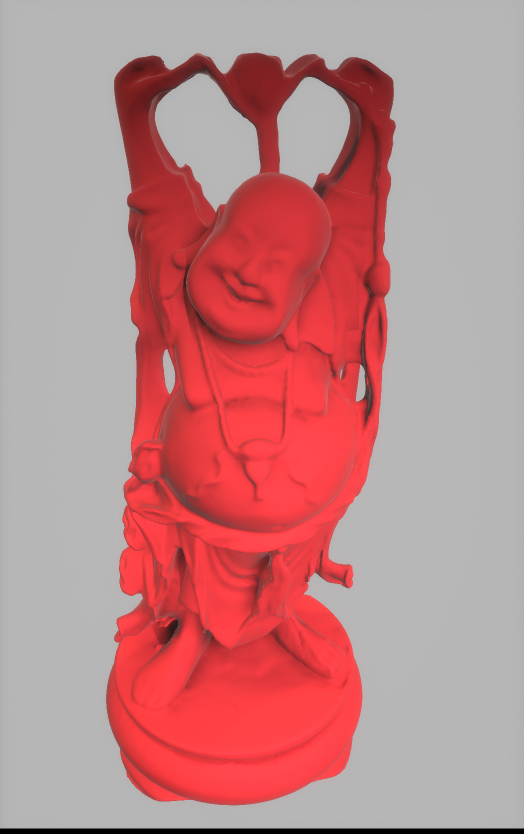
\includegraphics[width=0.3\linewidth]{./BRDFs/Lambert.jpg}}
  \subfigure[Blinn-Phong]{\label{fig:Buddha_BlinnPhong}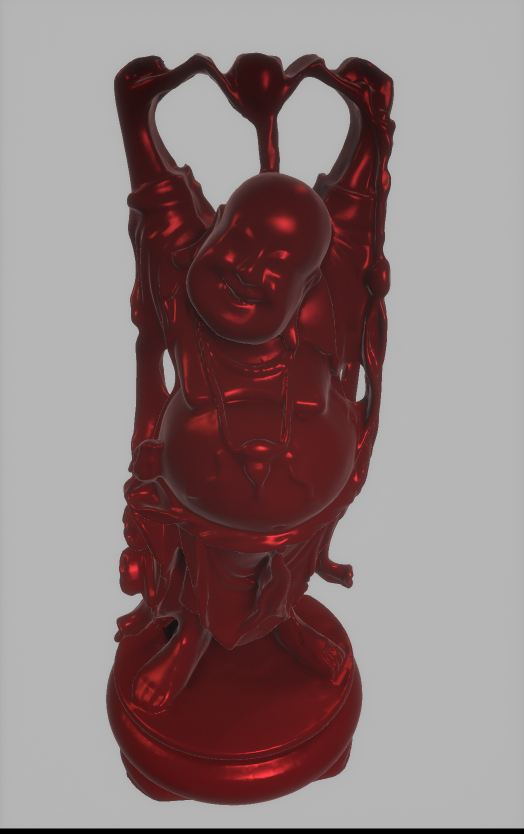
\includegraphics[width=0.3\linewidth]{./BRDFs/BlinnPhong_120.jpg}}
  \subfigure[Ashikhmin-Shirley]{\label{fig:Buddha_AS}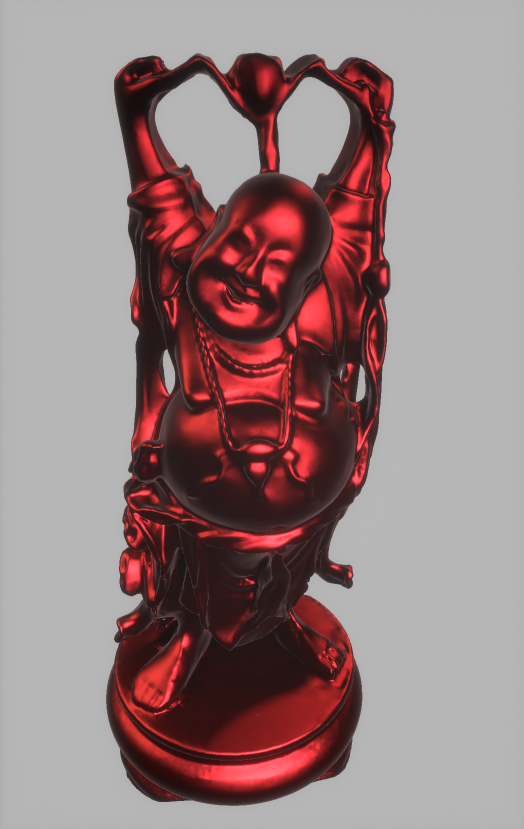
\includegraphics[width=0.3\linewidth]{./BRDFs/AS_f9_r1.jpg}}
\subfigure[Cook-Torrance]{\label{fig:Buddha_CT}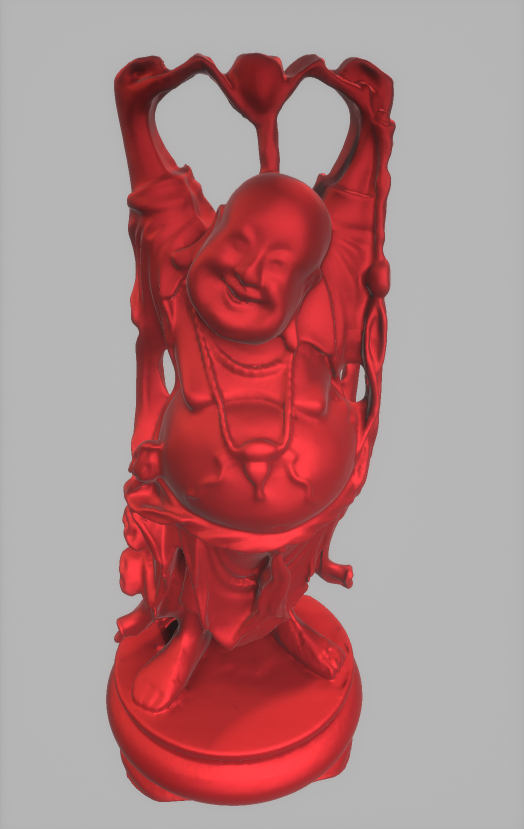
\includegraphics[width=0.3\linewidth]{./BRDFs/CookTorrance_f4_r9.jpg}}
\subfigure[ABC]{\label{fig:Buddha_ABC_area}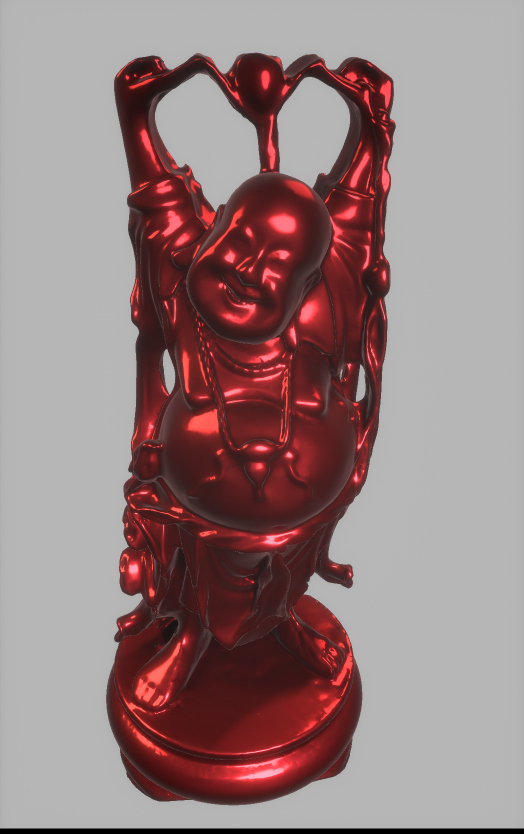
\includegraphics[width=0.3\linewidth]{./BRDFs/ABC_area_approx_b100_c99.jpg}}
\subfigure[ABg]{\label{fig:Buddha_ABg}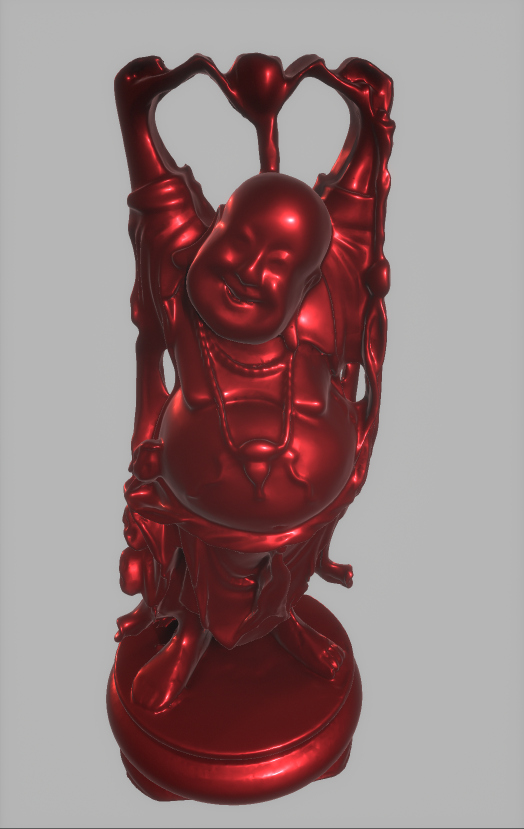
\includegraphics[width=0.3\linewidth]{./BRDFs/ABg_A06_B01_g19.jpg}}
  \caption{The effects of various reflection models on surface appearance}
  \label{fig:Buddha_reflectionModels}
\end{figure}

In order to introduce details into surfaces, the parameters to light reflection models can be made spatially-varying. For example, the Cook-Torrance model has a \emph{roughness} parameter which defines the width of specular highlights.  Finally, most BRDF models are parametrized with values by which components of the reflection should be scaled -- commonly one parameter for diffuse and one for specular reflectance.

The parameters influencing particular components of the reflection are intuitively called ``colors''. Even though the rendering equation is defined in terms of wavelengths and should be integrated over the entire visible spectrum, real-time computer graphics usually only concerns itself with light transport of three discrete bands. Due to practical considerations, the bands are the red, green and blue components of the \emph{sRGB} color space. Therefore any radiance calculations may be thought to operate on \emph{RGB} triplets, dubbed ``colors'' for the sake of simplicity.

\section{Rasterization}

Real-time rendering requires scenes to be described in a manner which is efficient in terms of storage and interpretation at run-time. Most commonly, objects are discretized as polygonal meshes with extra detail added in by two-dimensional images (called \textbf{textures}) parametrized onto the meshes. The former provide the macro structure of an object, whereas the latter cheaply represent fine detail wrapped over the mesh.

TODO: img

Such a vector-based representation may be visualized on a two-dimensional screen via the \emph{rasterization} algorithm. It is a \emph{forward} rendering algorithm (compared to \emph{backward} methods such as \emph{ray-tracing}) which starts from the scene primitives and via successive transformations, generates colors for the image. The major steps of the algorithm are:
\begin{enumerate}
\item \textbf{Transform} scene geometry into the coordinate space of the viewer.
\item Geometrically \textbf{clip} primitives to the viewable area in order to speed up the next stages and make sure no artifacts are produced.
\item \textbf{Scan-convert} primitives to pixels, calculate their colors and write into the target buffer.
\end{enumerate}
Variations of this algorithm have been used in real-time rendering applications since the beginning of computer graphics because it is simple and scales reasonably well with increasing scene complexity. Thanks to these traits combined with high demand for efficient and detailed rendering, rasterization has found its way into specialized hardware, and finally got integrated into display adapters.

Nowadays every desktop computer system, laptop and recently -- cellphone, contains a graphics card with a highly efficient implementation of the rasterization algorithm, capable of drawing millions of triangles per second, with high-end solutions delivering in excess of a billion triangles per second.

\section{Shading}

%TODO: comma?
Initially, hardware implementations of the rasterization algorithm were very constrained in terms of their functionality. Through a specialized API, such as \textbf{OpenGL} or \textbf{Direct3D}, the programmer could specify a set of textures to be mapped onto geometry, lights to influence it, and the actual geometrical data, which had to be transformed on the CPU side. The graphics card would then perform rendering computations according to a \emph{fixed-function pipeline}, combining the assigned textures in one of a few pre-specified ways, determining how lights influence geometry and perhaps applying a few other, rigid algorithms, such as fog simulation.

Such an approach was initially simple to implement in hardware, but as requirements in display fidelity rose, the number of custom algorithms designed to alleviate constraints of earlier custom algorithms skyrocketed. This resulted in messy APIs, unstable drivers, expensive hardware manufacturing and cumbersome programming against it. Gradually, \emph{programmable shading} was born.

The rasterization algorithm employed by current graphics cards is extensible through the use of programs which operate in various parts of its pipeline. \emph{Shaders} (as that is how they came to be known) provide a means of customizing the rendering, while still staying within the massively parallel implementation of the rasterization algorithm, as employed by GPUs \emph{(Graphics Processing Units)}. They are allowed to influence specific parts of the pipeline, therefore exist in several types. Each type, or \emph{domain} performs computations without referring to the other, in a strictly streamlined order. In case of hardware compliant with \emph{OpenGL 3.2} and \emph{Direct3D 10}, the shader types are are:
\begin{itemize}
\item \textbf{Vertex shaders} -- Execute for every vertex of the input provided to the GPU, they must provide positions of the vertex to be used in scan-conversion of primitives. Normally used to transform the input mesh from a local coordinate system into the space of the viewer, and then (normally through perspective or orthogonal projection) into a special homogeneous basis known as \emph{clip space}. Vertex shaders are a natural fit for deformation algorithms which do not require connectivity information, e.g. \emph{skinning} to make tissue and cloth move in accordance with a hidden skeleton of an articulated character. Another common use is image-based offsetting of vertices of a tessellated grid in order to render height-mapped terrain. Finally, vertex shader must produce all attributes which the next shader in the pipeline might require.
\item \textbf{Geometry shaders} -- An optional part of the rendering pipeline -- if enabled, resides between vertex and fragment processing. Whereas vertex shader operate on individual vertices of the input mesh and produce single vertices in a one-to-one mapping, geometry shaders run post \emph{primitive assembly} and operate on multiple vertices at a time, as well as on optional connectivity information. Moreover, they may output more (or fewer) than a single primitive, therefore being less constrained compared to vertex shaders. A geometry program might, for example, take a single triangle as an input, then subdivide it using a non-linear interpolation scheme and output multiple triangles. Or it might take a point and generate a polygon in its place.
\item \textbf{Fragment shaders} -- Also known as \textbf{pixel shaders}, they work on attributes interpolated from the output of vertex or geometry shaders. Executed for every pixel of the rasterized primitive, they compute the final color of the object, therefore usually performing \emph{texture mapping} and lighting computations.
\end{itemize}

When programmable shading was being introduced, the only way to perform it was by authoring assembly code to run on the GPU. It was also heavily constrained in terms of the number of instructions, registers and attributes it might use. With advancements in GPU technology, the limitations have been largely lifted or at least greatly reduced, e.g. allowing unlimited number of instructions to be evaluated per shader invocation. Several high-level specialized programming languages have also emerged, with the \emph{C}-like \emph{HLSL}, \emph{Cg} and \emph{GLSL} currently leading the pack.

%TODO: Say how changing shaders carries a cost, so we can't go wild. Also something about batching.

\section{Mental and hardware programming model mismatch}

Modern GPUs provide a very efficient model of computation allowing for creation of photorealistic renderings of three-dimensional scenes. Still, the programming model is not exactly the most intuitive one. The rendering equation does not feature vertex, geometry and fragment shaders either.

If we consider the elements that make up the rendering equation and the commonly used scene representation, then the logical elements emerge automatically. Under the aforementioned assumptions, we would ideally want to work with shader programs which describe:
\begin{itemize}
\item Light emission
\item Deformation and transformation of scene objects at the macro-scale
\item Materials applied to objects
\end{itemize}

Unsurprisingly, this separation of responsibility is used in many rendering systems which do not use the rasterization algorithm or simply do not run on commodity graphics hardware.

TODO: May use code generation to target the HW model, however shader permutation management issues pop up.
	TODO: Unity3D and Frostbite - Statically generate lots of shaders.
	TODO: Tri-Ace - Storing of shader permutations generated via play-testing instead of static generation of many combinations.

 % Introduction
%% Chapter 2

\chapter{ Problem statement }
\label{Chapter2}
\lhead{Chapter 2. \emph{ Problem statement }}

\section{Mental and hardware programming model mismatch}

We'd ideally want to work with geometry displacement, surface properties and light emission, not vertices and pixels.

Would like to work just on pixels, but vertex shaders must feed data to them and computations may be moved to the vertex stage for performance reasons.

Some stuff nicely done in vertex shaders, such as skinning.

Would like to work with materials, surfaces, lights

\section{Shader permutation management}

 We can map the mental model into the GPU model, but that requires some automation. Few systems make it workable.
 % Background Theory 
% Chapter 3

\chapter{ Related work }
\label{Chapter3}
\lhead{Chapter 3. \emph{ Related work }}

\section{Über- and micro-shaders}

A popular solution to the shader permutation problem is the \emph{ über-shader }. In this approach, the programmer creates a huge monolithic shader containing all the features a rendered object might need. Subsets of the functionality are then selected either at compile-time via preprocessor-based conditional compilation or at run-time via dynamic branching.

TODO: example

While conceptually simple and easy to implement, the über-shader approach is hard to debug and maintain. A more advanced take at the problem is to keep shader fragments separate and merge them conditionally using run-time logic or conservatively, yet statically generate permutations in the content pipeline. \citet{Hargreaves04} shows an approach based on runtime shader fragment combining. His implementation relies on a simple extension of the HLSL language in order to define the \emph{imports} and \emph{exports} of a shader fragment. Along with a special \emph{interface block}, a preprocessor is able to combine shader fragments together, linking their inputs and outputs. This effectively hides the complexity from the shader author, making maintenance and debugging easier. Hargreaves praises the robustness of this solution and mentions that it allows the usage of the same shader fragments in various rendering algorithms.

This work builds on shader fragment merging and extends it with automatic parameter type coercion and functional composition. I show how to implement such a scheme in a way that's easy to work with even for non-programmers.

% http://books.google.com/books?id=DgMSb_10l7IC&pg=PA555&lpg=PA555&dq=%22uber+shaders%22&source=bl&ots=-mu34jRtzO&sig=C3KIgqPIb6F8MDsOU0tSevVuN8M&hl=en&ei=zPZpTNGHNoGA4Aam1aHJCQ&sa=X&oi=book_result&ct=result&resnum=4&ved=0CCIQ6AEwAzgK#v=onepage&q=%22uber%20shaders%22&f=false

\section{RenderMan}

% TODO: the name is also a pun on Point Reyes

When designing a graphics rendering system, it is impossible not to bump into what currently constitutes the industry standard for film rendering -- RenderMan. Despite being over 20 years old, it continues to thrive as the benchmark for all rendering technology. It has been used in several dozen successful feature film productions and among its achievements is the first Oscar even awarded to the developers of a software package \cite{RenderManAwards}. An interesting aspect concerning RenderMan is that the overall structure of its Interface Specification (\emph{RISpec} in short) has survived mostly unchanged since its very first publication in 1988.

The rendering algorithm mainly utilized by Pixar's flagship implementation of RenderMan is called \textbf{REYES} (acronym for \emph{Renders Everything You Ever Saw}). It can be divided into the following steps:
	
\begin{enumerate}
\item \textbf{Bound} --- Conservatively cull off-screen objects using their bounding volumes. This early-out mechanism allows many calculations to be skipped for objects which can be trivially shown not to contribute to the final image.
\item \textbf{Split} --- Perform primitive-specific subdivision of the incoming geometry, generating more primitives as a result. Steps 1 -- 2 are evaluated recursively until the size of primitives meets a pre-configured threshold or a primitive declares that it is not splittable.
\item \textbf{Dice} --- Create a grid of \emph{micropolygons} from each primitive generated in the previous step. Each micropolygon is a quadrilateral approximately $^1/_2$ a pixel on a side. Micropolygons can be generated in a pattern matching the orientation of a texture applied to the primitive, enhancing quality via simplified filtering and improving performance due to access locality.
\item \textbf{Shade} --- Compute the lighting and shading at each vertex of the micropolygon grid.
\item \textbf{Sample} --- Generate the final image by stochastically sampling micropolygons for each pixel.
\end{enumerate}

It may seem that the algorithm is overly complex, especially when compared with regular rasterization, however it is able to exploit texture and geometric locality, parallelism and scales gracefully with increased scene complexity (\cite{Cook87reyes}). Stochastic sampling of micropolygons enables efficient computation of motion blur and depth of field effects. Finally, arbitrary primitive types are allowed, as long as they can be split or diced and finally converted into micropolygons.

The architecture is programmable via 5 \emph{shader} types (\cite{keyframeRSL1}):

\begin{description}
\item[Surface] --- Defines how a surface reacts to light, allowing the programmer to define its look. Surface shaders allow custom reflectance models to be defined, but also specify how the pigment or material of an object looks, hence allowing the definition of complete \emph{BRDF}s.
\item[Displacement] --- These shaders change the macro-structure of the surface, being able to alter normal vectors or offset the positions of micropolygons.
\item[Volume] --- Changes the color of light rays as they travel through a volume. May be used to create effects such as fog or smoke.
\item[Light] --- Represents the light source, allowing specification of light colors, shadows, intensity, falloff, ``barn door'' effects, etc. Computes the amount of lights which arrives at a particular point in space -- the surface being shaded.
\item[Imager] --- Imager shaders operate on image pixels just prior to the final output. They may be used e.g. to perform color correction or procedural background generation. Unfortunately, an imager shader being run for a single output pixel may only use the corresponding single pixel as an input, so more advanced effects, such as tone mapping (which require global or localized image statistics) are not feasible.
\end{description}

An important aspect of the RenderMan architecture is its ability to freely mix and match any primitives and shaders. Since every primitive eventually resolves to micropolygons, it can be used with any \emph{Displacement}, then processed by any \emph{Surface} shader. The latter may in turn interact with any \emph{Light} shaders, hence ensuring full orthogonality of the building blocks.

Unfortunately, micropolygon-based real-time rendering is still not viable for current commodity hardware. Nevertheless, there have been numerous attempts at an implementation. TODO: refs (render ants, a lot from Siggraph 2010). A prominent issue exists with the current GPUs not scaling well to sub-pixel-sized polygons, resulting in up to 8 times more shading work than what would seem to be required (TODO: ref).

Still, even without using micropolygon-based rendering, an architecture can be developed which retains some of the advantages RenderMan possesses. In particular, this thesis presents a shading framework decoupled from the domains imposed by current GPUs, instead being closer to the model employed by RenderMan. Additionally, the limitation of \emph{Imager} shaders is lifted, hence enabling more sophisticated post-processing effects to be created.


\section{Deferred rendering}

The standard \emph{Forward} rasterization algorithm requires that material and light shaders for an objects be merged into a single GPU program. The implications are two-fold:
\begin{enumerate}
\item The lower bound on the number of GPU programs that need to be compiled is $O(m * l)$ (where $m$ stands for the number of materials and $l$ for the number of light shader \emph{combinations}), or \emph{multi-pass} rendering must be used.

The number of shaders created this way may be prohibitively large. One obvious workaround is to restrict the possible light shader combinations. This may be achieved via über-lights \cite{UberLights, UberLightsCg} or just constraining the renderer to a handful of light types. A related technique is to use a shader designed for more lights than what's necessary and zero-out any excessive light slots. For instance, when the renderer must render an object influenced by two point-lights, it may use a shader for rendering it with three point-lights, assuming zero intensity for one of the parameters. Naturally, this approach, just like the über-light one, carries a runtime cost which may be prohibitive in a complex setup.

An alternative solution to this issue is \emph{multi-pass} rendering, where the object is rendered once for an affecting light, and the resulting per-fragment irradiance is summed via additive blending. The downside is that in scenes with complex geometry, rendering objects multiple times will quickly drain the computational budget.

\item Lights can only influence the scene at the granularity of individual objects, not their vertices or rasterized pixels. Even when a light would affect a small part of an object, it must be evaluated for all elements thereof, because a single \emph{batch} may only use a single shader per domain.

Splitting objects into smaller pieces might be an option, however GPU batch submission carries a nontrivial cost \cite{BatchBatchBatch}, hence the tendency is to do the exact opposite and pack multiple objects into shared batches.
\end{enumerate}

Recently a technique known as \emph{deferred shading} has been gaining popularity, as it offers an elegant solution to both of these problems. Originally proposed in \citet{DeeringDeferred}, the algorithm separates the rendering pipeline into two stages:

\begin{enumerate}
\item Render surface attributes of the visible scene into a set of framebuffers \emph{(collectively called the \textbf{G-buffer})}.
\item For each light, evaluate its contribution on the surfaces encoded within a subset of the \emph{G-buffer}.
\end{enumerate}

Of the two passes, only the first one requires the actual geometry of the scene to be rendered and material shaders evaluated. Similarly, the second pass only runs light shaders. Importantly, each light can be treated separately from another and from material shaders, eliminating the need for merging light and material code -- the main source of the combinatorial explosion of vertex and pixel shaders.

The main strength of deferred shading is at the same time the root of a drawback. Since the second pass only runs light shaders and has no knowledge of the source objects which contributed to the \emph{G-buffer}, it may no longer run per-object shader code. When all objects are just samples in the \emph{G-buffer}, there is no clear way of supporting per-object reflection models.

Another tricky issue is that of translucency. Because the \emph{G-buffer} may only store properties of a single surface at a single fragment location, it doesn't handle translucency in a natural fashion. \citet{HumusDeepDeferred} demonstrates an approach using depth peeling, which is able to overcome this limitation. He uses texture arrays to encode attributes of multiple depth layers. The second pass of deferred shading then computes light influence on each of these layers, stopping on opaque surfaces. This results in good performance for typical scene configurations, since most will have far more opaque elements than translucent ones. The main downside of his approach is the fact that the technique requires $n$ G-buffers in order to support $n$ depth layers, putting much strain on memory.

A more common approach for handling translucency is to render non-opaque surfaces in a separate pass using a traditional forward rendering algorithm. Using read-only depth testing against a depth buffer containing the opaque parts of the scene, translucent surfaces can be blended into the result of deferred shading. A major inconvenience this approach entails is having to maintain both a deferred and a forward renderer, along with material and light shaders which might be used in both of them. The rendering system presented in this work makes it relatively easy by allowing the same \emph{material}, \emph{light}, \emph{reflectance} and \emph{structure} shaders (or \emph{kernels} in its nomenclature) to be used in any of the implemented rendering algorithms.

\subsection{Deferred lighting}
\label{sec:DeferredLighting}

% TODO: ref the olde nvidia paper
The regular deferred rendering algorithm requires a large G-buffer, which in some cases may be prohibitive due to memory capacity or bandwidth constraints. \citet{Engel08PrePass} proposes an alternative approach, currently known \emph{light pre-pass}, \emph{deferred lighting} or \emph{pre-lighting}. Unlike classical deferred rendering, which consists of two phases, this algorithm is composed of three stages:

\begin{enumerate}
\item Render a minimal \emph{G-buffer}, containing the surface depth and normal.
\item For each light, evaluate its contribution on the surfaces encoded within a subset of the \emph{G-buffer} using only the reflectance model.
\item Render scene objects again, this time fully evaluating their materials and combining them with the illumination computed in the previous step.
\end{enumerate}

Such a breakdown of rendering operations trades extra geometric cost for less G-buffer memory utilization, which in particular scene configurations and platforms translates into faster execution.

% http://http.developer.nvidia.com/GPUGems2/gpugems2_chapter09.html

\section{Graph-based systems}

Creating immersive environments requires many complex shaders. \citet{Tatarchuk06ToyShop} mentions that the ``Toy Shop'' demo (shown in figure \ref{fig:ATItoyshop}) contained about 500 custom shaders, so this number can only be expected to be higher in a complete game. It must therefore be easy to create custom shaders, and it must be straightforward for artists in particular.

\begin{figure}[h!]
  \centering
    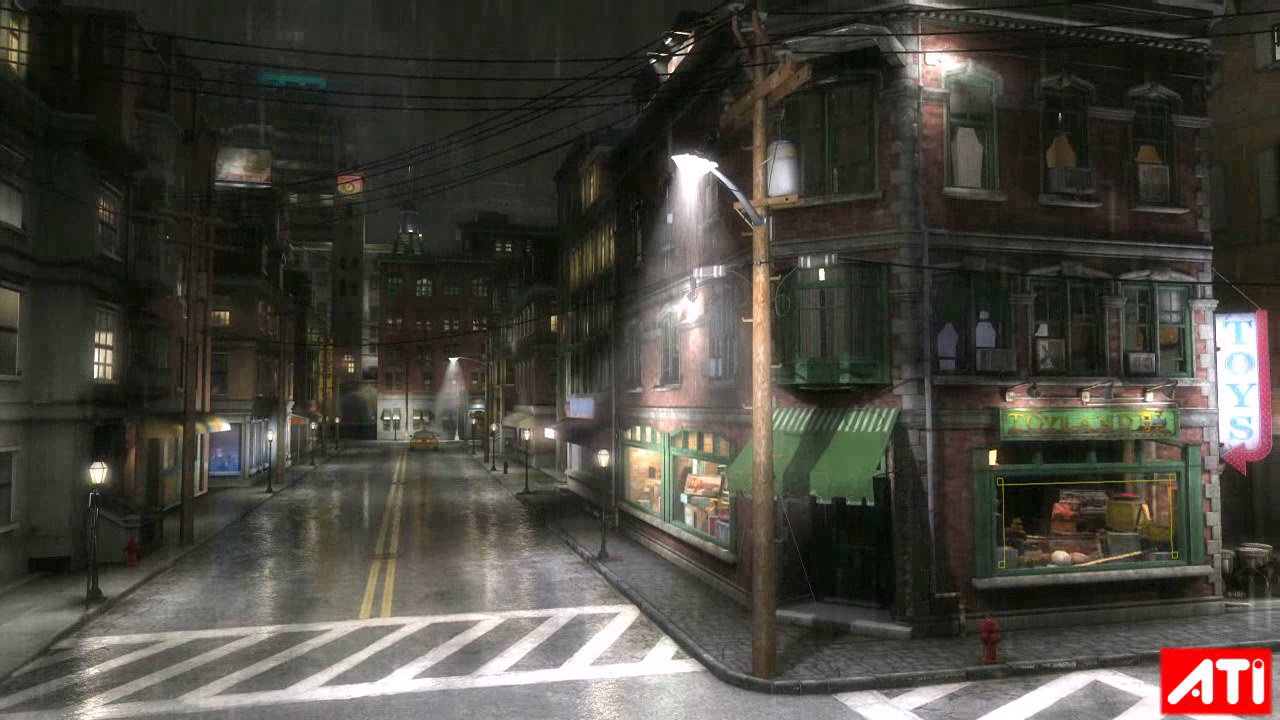
\includegraphics[width=0.9\linewidth]{./Chapters/ati-demo-toyshop.jpg}
    \caption[ToyShop demo]{AMD's real-time Toy Shop demo utilizes about 500 custom shaders. Image courtesy of AMD Graphics Product Group}
  \label{fig:ATItoyshop}
\end{figure}

% http://udn.epicgames.com/Three/MaterialsTutorial.html
% Frostbite, Project Offset, Maya Hypershade, 
A popular approach for enabling artists to easily create shaders is to use a graph-based editor, in which computations and data are represented by nodes. The list of implementations of such systems is getting consistently longer, since despite some shortcomings \cite{ChristerGraphShaderEditorsSuck}, they empower artists to create rich content swiftly, instead of having them rely on programmers for all shaders. This subsequently reduces the communication overhead and takes the load off programmers, resulting in faster product development.

Nevertheless, graph-based shader editors are no silver bullet, do not completely remove the need for efficient communication in a team and must still be designed with care. Simply moving all shader computations into a graph-based representation only turns regular text-based code entry into visual programming, an area which hasn't been adequately explored for production environments.

When \citet{AbramWhitted90} introduced the first visual shader authoring tool, they expressed concern about the possibility of type mis-matches within the data being manipulated by graph-based programs. Indeed, in order to avoid visual clutter, most graph-based tools hide type information of inputs and outputs within nodes. Furthermore, \citet{mcguire2006shadetrees} points out that this mis-matching issue extrapolates onto semantic meaning of data:
	
\begin{quote}
In fact, this problem extends beyond storage types to interface mismatches between atoms, e.g., assumptions like “the light vector has unit length” or “RGB values are pre-multiplied by the alpha channel.” It is almost impossible for the user to ensure that the types are correct when the programming tool conceals those types. 
\end{quote}

In a summary, a graph-based shader authoring tool should not be implemented in a naïve manner. Doing so means that neither artists nor programmers are able to use it effectively. Another important point to note is that if a graph-based shader authoring tool only allowed, for instance, direct pixel shader editing, then the vertex shader would need to be kept in sync in some way. Hence the second goal besides solving type mis-match issues is a paradigm shift, one which frees the artists from the subdivision imposed by the GPU architecture.

One example of a renderer which decouples artists from thinking in terms of vertex and pixel shaders is \emph{Frostbite}. In \cite{AT07}, Andersson details that their approach uses graph-based \emph{surface} shaders. Similarly to the ones in \emph{RenderMan}, they decouple material properties from lighting, environment and geometry. All shaders are treated as content instead of code, and as a part of the pipeline, converted to an efficient representation for run-time processing. The \emph{Frostbite} engine has to date been used in a few large games, running on the PC, Xbox and PS3 platforms, being a testament to the practicality of the solution.

\subsection{Abstract Shade Trees}

\citet{mcguire2006shadetrees} introduce \emph{Abstract Shade Trees} which tackle the type mismatch problem \cite{AbramWhitted90} in an interesting manner. The key concept their paper introduces is embedding \emph{semantic} information in types used to define the interfaces of computational atoms. They subsequently use a \emph{weaver} algorithm to automatically connect atoms and perform type coercions.

They note that regular types used by a shading language such as GLSL are "merely C-style storage specifiers with little value as abstractions. For example, a color, a 3D location, and a row of a 3×3 matrix have the same type, which is also indistinguishable from an array of three floating-point numbers." On the other hand, their \emph{semantic types} are able to carry more meaningful information, such as:
\begin{itemize}
\item The \textbf{Basis} in which instances of this type are defined (tangent, object, world, screen).
\item \textbf{Length} of a vector (unit, any).
\item The very interpretation, e.g. whether it's a color, a texture coordinate or a normal vector.
\end{itemize}

Such a type system allows stronger checking, but it also enables automating tedious tasks such as coordinate-space conversions. For example, when one atom outputs a position vector in \emph{object} space, and another requires the position in \emph{world} space, it becomes possible to generate code to perform the required math.

\begin{figure}[h!]
  \centering
    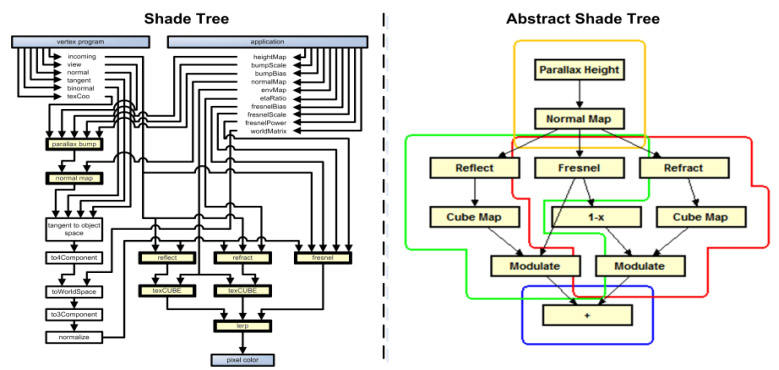
\includegraphics[width=0.9\linewidth]{./Chapters/AbstractShadeTree.jpg}
    \caption[Abstract Shade Tree]{A conventional Shade Tree (left) and the equivalent Abstract Shade Tree (right). Image courtesy of McGuire et al.}
  \label{fig:AbstractShadeTree}
\end{figure}

An \emph{Abstract Shade Tree} is normally much more compact than an equivalent \emph{conventional Shade Tree}, as demonstrated by Figure \ref{fig:AbstractShadeTree}. Thanks to the complexity hiding, shader authoring becomes less error prone and especially easier for users who do not have knowledge of programming concepts such as types, variables or the vector math used to implement algorithms inside atoms.
 
The rendering system presented in this work utilizes a \emph{semantic type system}. In contrast to Abstract Shade Trees, automatic determination of fine-grained dependencies between atoms is not central to its function. Manual connections of inputs and outputs are allowed in addition to setting coarse-grained dependencies. Both the former and the latter are then subject to automatic type coercions, hence type safety is retained. The work of McGuire et al. is also extended by the introduction of \emph{semantic expressions}, which provide parametric polymorphism and basic type algebra for atom parameters.

% TODO: in the next section, note how parametric polymorphism is provided % Previous work
% Chapter 4

% TODO: something about the CPU-side of things

\chapter{ Nucleus }
\label{Chapter4}
\lhead{Chapter 3. \emph{ Nucleus }}

This chapter contains a description of the internal structure of a rendering system created for the purposes of this thesis, henceforth called ``\textbf{Nucleus}.'' After a brief overview of the major components in the following section, the building blocks used therein are presented. Finally, the chapter provides an in-depth look at the internal manipulation of the basic elements and how they are optimized and translated into a form which the underlying GPU can understand.

\section{Overall structure}

At the highest level, the architecture of Nucleus is split in two layers.
\begin{itemize}
\item The first layer completely wraps an underlying rendering API, providing primitives which are easier to use and less error-prone, while retaining high efficiency.
\item The second layer is the high-level rendering interface which is the main topic of this thesis, described in further detail in this chapter.
\end{itemize}

\begin{figure}[ht!]
  \centering
    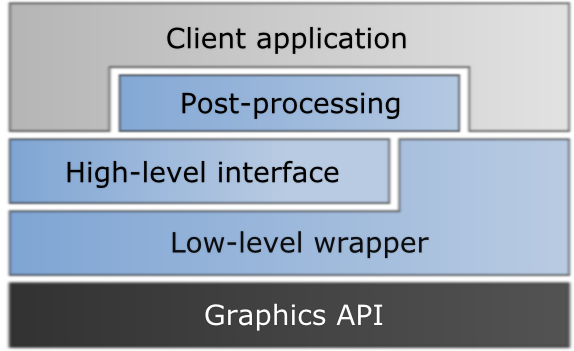
\includegraphics[width=0.5\linewidth]{./Figures/layers.png}
    \caption[Nucleus Layers]{The top-level composition of Nucleus.}
  \label{fig:nucleusLayers}
\end{figure}

Aside the above, Nucleus offers a post-processing framework, which in turn may use both of these layers.

\section{Low-level abstraction layer}
\label{sec:lowLevelInfo}

The high-level machinery of Nucleus may be built directly on top of a rendering API such as OpenGL or Direct3D, however a wrapper over these is desirable for numerous reasons:

\begin{enumerate}
\item The OpenGL API is portable and supported by multiple operating systems, however its implementation in drivers is currently less stable than that of Direct3D. Hence it is vital to be able to support both APIs.
\item Hardware may support rendering APIs to varying degrees via feature sets and extensions, yet workarounds can be created and exposed as a common set of features. Additionally, functionality required by the standards is implemented to varying degrees, and sometimes contains bugs. The wrapper allows these exceptional details to be caught in a single location.
\item Directly working with the graphics API is error-prone and may be difficult to debug. The wrapper can enforce particular usage patterns, allow straightforward resource management and reduce code duplication, all of which lead to faster and cheaper development.
\end{enumerate}

The lowest abstraction layer has been built on a level similar to Microsoft's XNA library and currently has a backend utilizing \emph{OpenGL 3.3} and NVIDIA's \emph{Cg Toolkit}. The main building blocks of the framework are:

\begin{description}

\item[Effect] --- wraps vertex, geometry and fragment shaders together, allows shader specialization (e.g. setting the implementations of Cg interfaces, providing sizes for unsized Cg arrays). Once compiled, allows the programmer to provide values for uniform parameters shared by all instances of the effect. Finally, it allows instantiation into EffectInstances.

\item[EffectInstance] --- provides a name space and storage for uniform and varying parameters associated with a single instance of an Effect. Additionally, uses a VertexArray to cache current varying parameter bindings. Automatically performs reference counting of resources assigned as uniform (Textures) and varying parameters (VertexBuffers). The memory for EffectInstances is allocated from pools in contiguous slabs for both the structure data and the effect-dependent payload. By adding an indirection to parameter storage, multiple Effects and EffectInstances may source their parameters from the same variable in memory, possibly managed entirely by the client. Typically, each object in the scene will own a single EffectInstance for each Effect it may be rendered with.

\item[Buffer] ---allows the specification and modification of graphics API-allocated memory (VRAM, AGP, system).

\begin{description}
\item[VertexBuffer] --- used for generic untyped vertex attributes. The actual types are specified when binding varying parameters to EffectInstances and specifying the offset, stride and type of the underlying data.
\item[IndexBuffer] --- specialized for 16 and 32-bit mesh indices.
\item[UniformBuffer] --- bindable uniform / constant buffers for shader programs.
\end{description}

\item[VertexArray] --- a special kind of a driver-level object that caches varying parameter bindings, allowing for reduction of API calls.

\item[Framebuffer] --- wrapper over all classes of framebuffers with automatic usage of Multiple Render Targets, rendering to textures, floating point support, etc.

\item[Texture] --- provides access to 1D, 2D, 3D, rectangle and cube texture maps, updating and querying their data.
\end{description}

The aforementioned resources are accessed via opaque handles created and managed by a \textbf{Renderer}, eliminating the potential of fatal user mistakes such as manual disposal of a resource and its subsequent usage or memory corruption. For example, calling \emph{createVertexBuffer(\ldots)} on a \emph{Renderer} instance yields a \emph{VertexBuffer} instance with meaningful access methods, such as \emph{mapRange} and \emph{setSubData} -- it is however only a thin \textbf{struct} wrapping a resource handle. The methods within it only pass the parameters along with the handle to the API provided by the \emph{Renderer}.

Additionally, the \textbf{Renderer} provides functionality to create, dispose and render the contents of a \textbf{RenderList} according to the current \textbf{RenderState}.

The \textbf{RenderList} is a collection of indices (ordinals) of EffectInstances and basic associated data required to render them, including:
	
\begin{itemize}
\item Model $\rightarrow$ world and world $\rightarrow$ model transformation 4×3 matrices
\item An IndexBuffer along with the count of indices to use, offset, min and max therein
\item The number of instances of the object to be rendered via \emph{hardware instancing}
\item Mesh topology
\end{itemize}

An important factor to note is that the RenderList does not plainly contain EffectInstances, but rather their \emph{rendering ordinals}. The ordinals are 32-bit numbers assigned to each effect instance and managed internally by the renderer. Their order is determined by a heuristic attempting to minimize the number of state changes required when rendering the instances. This means that once the render list is constructed, the algorithm to minimize the required state changes basically boils down to \emph{sorting the ordinals}, which is a cheap operation. More ordering options will be made available in the future, so that the objects may be sorted by distance or using per-Effect routines built with knowledge of their performance characteristics.

\begin{figure}[ht!]
  \centering
    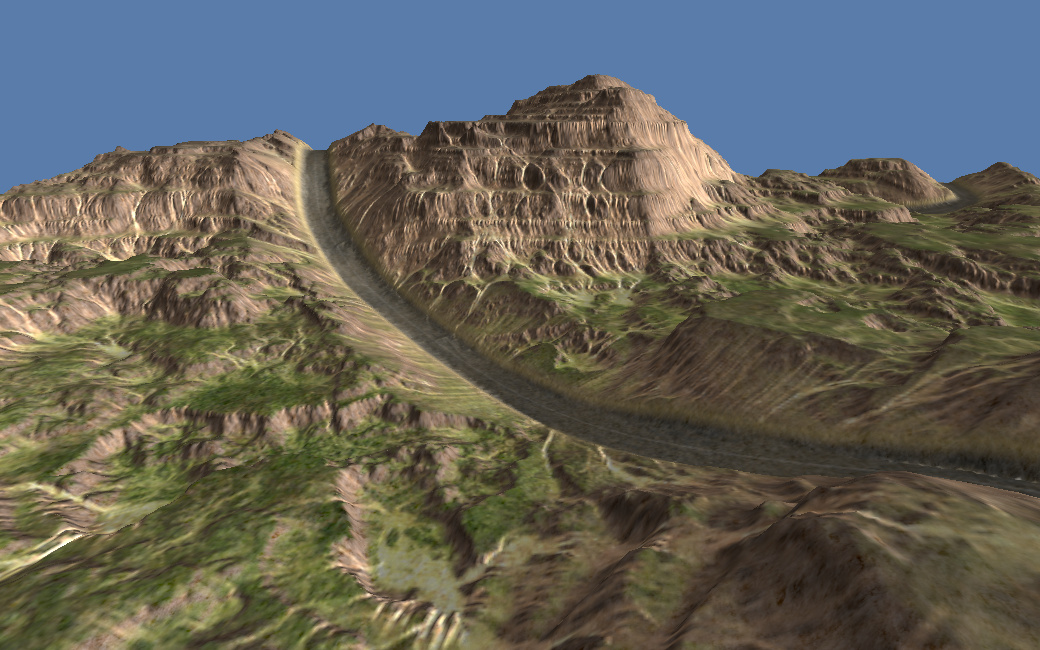
\includegraphics[width=0.9\linewidth]{./Figures/terrainRendering.jpg}
    \caption[terrainRendering]{A terrain example implemented using the low-level rendering API wrapper.}
  \label{fig:terrainRendering}
\end{figure}

As mentioned before, the \textbf{Renderer} also gives access to the \textbf{RenderState}, a set of common rendering settings, such as the mode of depth-testing, blending, back-face culling, etc.

The graphics base layer can therefore be used instead of the underlying graphics API, completely hiding its complexity and error-prone setup. It also makes it possible to change the backend without touching client code. The following is a code fragment of a Chunked LoD \cite{chunkedLoD} terrain rendering example (shown in \fref{fig:terrainRendering}) implemented using the low-level interface only:

\noindent\begin{minipage}{\textwidth}
\begin{lstlisting}[frame=single]
efInst = renderer.instantiateEffect(effect);
EffectHelper.allocateDefaultUniformStorage(efInst);

vb = renderer.createVertexBuffer(
	BufferUsage.StaticDraw,
	cast(void[])positions
);
va = VertexAttrib(
	0,
	vec3.sizeof,
	VertexAttrib.Type.Vec3
);

final vdata = efInst.getVaryingParamData("VertexProgram.input.position");
vdata.buffer = &vb;
vdata.attrib = &va;
\end{lstlisting}
\end{minipage}

The above sample instantiates an \emph{Effect} containing a vertex and a fragment shader, then creates a vertex buffer and finally binds a varying parameter in the vertex shader to a portion of that buffer. Such code would be considerably longer if the underlying OpenGL and Cg APIs were used instead.
	
\section{Kernels}
\label{sec:Kernels}

The basic building block of the high level rendering interface of Nucleus is called a \emph{kernel}. Conceptually, it is just a function. The implementation of a kernel may be specified using a code snippet (the current implementation allows the \emph{Cg} language for this purpose). The more interesting option is to define it using a graph. Specifically, a directed acyclic graph whose nodes are either kernels or special-purpose entities. The special-purpose nodes can be used to denote what constitutes the input and output parameters of a graph-based kernel, as well as to request external data for it.

While first-class support of graphs does not result in more expressive power than that of regular function-based composition, it provides a comfortable mental and programmatic framework for such composition. It enables the use of classical graph algorithms and makes development of authoring tools easier.

As a convention, the return values of kernels are called \emph{output parameters} and denoted by the \textbf{out} keyword in the kernel signature. Conversely, regular kernel parameters are called \emph{input parameters} and optionally denoted by the \textbf{in} keyword. This is modeled after the \emph{Cg} shading language.

Within a kernel graph, connections may exist between nodes, as well as between particular parameters of the nodes. The implications of this decision are discussed further in this chapter.

\subsection{Standard kernel types}

Similarly to how GPU-based shading requires the specification of shader programs for each of the processing domains (vertex, geometry an fragment), Nucleus demands that a kernel be provided for each of \emph{its} domains. The major difference lies in what the domains are. Each object to be rendered within Nucleus must have 3 kernels specified for it:

\begin{description}
\item[Structure] --- Defines the macro-structure and mostly contains what a vertex or geometry shader might. It is responsible for providing the primitives to be rendered, including data such as positions, normals, partial derivatives of position with respect to texture coordinates, etc.

\item[Reflectance] --- Enables the object to interact with lights by implementing a reflection model. Examples include the Lambertian model, Blinn-Phong, Cook-Torrance and Ashikhmin-Shirley, all of which have been implemented in Nucleus.

\item[Material] --- This is the level on which most artists will work, specifying the albedo of the rendered object, its bumpiness, specular tint, emissive lighting, roughness, etc. Kernels of this type will be created for types of objects in a scene, as well as for particular instances thereof.
\end{description}

Specifying these kernels for a renderable object boils down to designating a \emph{concrete} kernel with a compatible signature for each of the above \emph{abstract} kernels.

A scene will usually also contain lights, each of which must be associated with a kernel. In this case, an implementation of the abstract \emph{Light} kernel. At program runtime, \emph{Light} kernels are connected to the per-object \emph{Reflectance} kernels. This mechanism allows specification of custom attenuation, sampling and shadowing algorithms, which automatically are applicable to any \emph{Reflectance} kernel.

% TODO: link to info about the signatures of these kernels in some other chapter

Such a break-down of domains may superficially look similar to the shader types GPUs require. \emph{Structure} kernels resemble \emph{vertex} shaders, \emph{Material} kernels resemble \emph{pixel} shaders. The first major distinction is that the signatures of the above kernels are fixed in Nucleus, hence each Material may be combined with any Reflectance, any Structure and any Light. The second important difference is that these kernels are not tied to any particular part of the pipeline. Instead, a \emph{Renderer} is free to use these kernels in any rendering algorithm, as detailed in \sref{sec:Renderers}.

Another core kernel type is used in \emph{post-processing} operations and described in \sref{sec:PostProcessing}.

This particular breakdown of processing domains is comparable to the \emph{RenderMan} model:

\begin{center}
\begin{tabular}{ | c | c | c | }
\hline
RenderMan shader & Nucleus kernel \\
\hline
Surface & Material + Reflectance \\
Light & Light \\
Imager & PostProcess \\
Displacement & Structure \\
Volume & --- \\
\hline
\end{tabular}
\end{center}

Requiring that material and reflectance be defined by separate kernels gives Nucleus the ability to split the rendering equation into independent components and apply algorithms which utilize this distinction for performance gains in complex scene configurations -- for example, Sections \ref{sec:ForwardRenderingExample} and \ref{sec:DeferredLightingExample} demonstrate how it allows Nucleus to use the same kernels for \emph{Forward} and \emph{Deferred} rendering, respectably. While it restricts the freedom of an artist to some extent, real-time rendering systems used in large, commercially successful computer games have often been limited to just a \emph{single} reflectance model \cite{CryEngine3Deferred, Killzone2Deferred}.

There is currently no support whatsoever for volume shaders in Nucleus. A proper solution would require ray marching in volumes and is beyond the scope of this thesis.

\section{Semantic type system}

% TODO: ref the related work section? maybe put semantic types into an index?
Nucleus uses \emph{semantic types} in order to describe the signatures of computational kernels. Each type is a set of \emph{trait} values and each \emph{trait} is an enumerated type in the classical meaning used in programming languages. Possible traits and their values include:
\begin{description}
\item[basis] --- The coordinate space of a vector: model, world, view, clip, tangent,
\item[colorSpace] --- RGB, sRGB, logLUV, etc.,
\item[unit] --- Whether the magnitude of a vector equals one: true, false,
\item[linearity] --- linear, logarithmic, exponential, etc.,
\item[use] --- What instances of this type are to be used for: position, normal, color, uv, etc.,
\item[type] --- The underlying plain type in the target language: float, float2, float3, float4, int, bool, sampler2D, etc.
\end{description}

Trait values of the same name are considered distinct if they belong to different traits. For example, value \emph{A} of trait \emph{X} is distinct from value \emph{A} of trait \emph{Y}. In order to make the definition mathematically sound, a trait value may be considered a $(trait, value)$ tuple.

A type is then any combination of trait values, e.g. \emph{``type float3 + use position + basis world''} and \emph{``type float2 + use uv''}, where the ``+'' sign denotes a delimiter (actually, a semantic expression operator, as further described in \sref{sec:SemanticExpressions}). An empty set of trait values is a valid type as well.

\subsection{Type coercion}
\label{sec:TypeCoercion}

A kernel graph specified by the user or constructed by an algorithm must be type-checked within Nucleus before it is used in any rendering operation. This section first explains the process for individual connections, then extends it to entire kernel graphs.

Given a connection from an output parameter of type $X$ to a input parameter of type $Y$, the connection is determined to be valid if $Y \subseteq X$. Otherwise such a connection is a type mismatch. For example, connecting an output parameter of type \emph{``type float3 + use position''} to an input parameter of type \emph{``type float3''} is valid, however connecting \emph{``type float4''} to \emph{``type float3''} or to \emph{``type float4 + use color''} is a mismatch.

In the case of a mismatch, Nucleus will try to perform \emph{type coercion} by inserting additional computational kernels between the source and the destination. The kernels which it considers come from a specifically designated set of \emph{semantic converters}. Each semantic converter is a kernel of a single input and a single output parameter. Additionally an integral \emph{cost} value is associated with each converter, which is an estimate of the computational complexity of the code within its definition.

\begin{figure}[ht!]
  \centering
    \digraph[width=0.9\linewidth]{SemanticSearchGraph}{
		"1" [ fillcolor = "\#d0ffd0" label=<<font color="\#1040a0" >use</font> normal<br/><font color="\#1040a0" >basis</font> model> ];
		"1a" [ label=<<font color="\#1040a0" >use</font> normal<br/><font color="\#1040a0" >basis</font> model<br/><font color="\#1040a0" >unit</font> true> ];
		"2" [ label=<<font color="\#1040a0" >use</font> normal<br/><font color="\#1040a0" >basis</font> world> ];
		"2a" [ label=<<font color="\#1040a0" >use</font> normal<br/><font color="\#1040a0" >basis</font> view> ];
		"2b" [ label=<<font color="\#1040a0" >use</font> normal<br/><font color="\#1040a0" >basis</font> clip> ];
		"3" [ fillcolor = "\#d0ffd0" label=<<font color="\#1040a0" >use</font> normal<br/><font color="\#1040a0" >basis</font> world<br/><font color="\#1040a0" >unit</font> true> ];
		"1" -> "2" [ label="modelToWorld" ];
		"1" -> "1a" [ label="normalize" ];
		"2" -> "2a" [ label="worldToView" ];
		"2a" -> "2b" [ label="viewToClip" ];
		"2" -> "3" [ label="normalize" ];
	}
    \caption[Implicit semantic search tree]{An example slice of the implicit semantic conversion graph.}
  \label{fig:SemanticSearchGraph}
\end{figure}

It is possible to define a directed weighted graph $G=(V, E)$ such that its vertices, $V$ are all the possible semantic types. The graph contains an edge $e$ from $a$ to $b$ if and only if there exists a converter, which turns type $a$ into a type which may be connected to type $b$ without a mismatch. The weight associated with $e$ is the cost value of the corresponding converter.

Because $G$ contains all possible semantic types, it must contain $X$ and $Y$. A search for the shortest path is performed using Dijkstra's algorithm. A fragment of the implicit search tree is visualized in \fref{fig:SemanticSearchGraph}. If a path from $X$ to $Y$ in $G$ does not exist, an error is reported. If two or more shortest paths are found, an ambiguity error is reported. Otherwise, the path defines a valid \emph{type coercion}. New nodes are created within the kernel graph and inserted in place of the original parameter connection.
	
\subsection{Automatic connection determination}

The kernel graph may contain connections not only between particular parameters, but also between nodes. The type-checking process converts these coarse-grained dependencies into individual parameter connections using an extension of the type coercion algorithm.

\begin{figure}[ht!]
  \centering
  \subfigure[Coarse dependency between nodes]{\label{fig:AutoSemanticGraph1}\digraph[width=0.7\linewidth]{AutoSemanticGraph1}{
    		"src" [
    			shape=rectangle style="rounded,filled"
    			label = <<table border="0" cellborder="0" cellspacing="8" >
    			<tr><td port="main" ><font point-size="14" >Source</font></td></tr>
    			<tr><td port="p1" ><font color="\#1040a0" >use</font> position + <font color="\#1040a0" >basis</font> model</td></tr>
    			<tr><td port="p2" ><font color="\#1040a0" >use</font> normal + <font color="\#1040a0" >basis</font> model</td></tr>
    			<tr><td port="p3" ><font color="\#1040a0" >use</font> color</td></tr>
    			</table>>
    		];
    		"dst" [
    			shape=rectangle style="rounded,filled"
    			label = <<table border="0" cellborder="0" cellspacing="8" >
    			<tr><td port="main" >Destination</td></tr>
    			<tr><td port="p1" ><font color="\#1040a0" >use</font> position + <font color="\#1040a0" >basis</font> world</td></tr>
    			<tr><td port="p2" ><font color="\#1040a0" >use</font> normal + <font color="\#1040a0" >basis</font> world + <font color="\#1040a0" >unit</font> true</td></tr>
    			<tr><td port="p3" ><font color="\#1040a0" >use</font> color</td></tr>
    			</table>>
    		];
    		src -> dst;
	}}
  \subfigure[The resulting fine-grained connections and conversions]{\label{fig:AutoSemanticGraph2}\digraph[width=0.9\linewidth]{AutoSemanticGraph2}{
    		"src" [
    			shape=rectangle style="rounded,filled"
    			label = <<table border="0" cellborder="0" cellspacing="8" >
    			<tr><td port="main" ><font point-size="14" >Source</font></td></tr>
    			<tr><td port="p1" ><font color="\#1040a0" >use</font> position + <font color="\#1040a0" >basis</font> model</td></tr>
    			<tr><td port="p2" ><font color="\#1040a0" >use</font> normal + <font color="\#1040a0" >basis</font> model</td></tr>
    			<tr><td port="p3" ><font color="\#1040a0" >use</font> color</td></tr>
    			</table>>
    		];
    		"dst" [
    			shape=rectangle style="rounded,filled"
    			label = <<table border="0" cellborder="0" cellspacing="8" >
    			<tr><td port="main" >Destination</td></tr>
    			<tr><td port="p1" ><font color="\#1040a0" >use</font> position + <font color="\#1040a0" >basis</font> world</td></tr>
    			<tr><td port="p2" ><font color="\#1040a0" >use</font> normal + <font color="\#1040a0" >basis</font> world + <font color="\#1040a0" >unit</font> true</td></tr>
    			<tr><td port="p3" ><font color="\#1040a0" >use</font> color</td></tr>
    			</table>>
    		];
    		src:p1 -> dst:p1 [ label="modelToWorld" ]
    		src:p2 -> dst:p2 [ label="modelToWorld, normalize" ];
    		src:p3 -> dst:p3;
	}}
  \caption[Automatic connection determination example]{A simple graph in which a dependency between nodes is specified in order to be resolved by the automatic connection determination algorithm into individual parameter connections.}
  \label{fig:AutoSemanticGraph}
\end{figure}

To automatically determine the parameter which should be connected to an input of a kernel graph node, all output parameters of all nodes connected to this node are considered. The possible type coercions are evaluated in parallel and the shortest one is selected. Similarly to the aforementioned algorithm, an ambiguous choice is an error. An example of this process is shown in \fref{fig:AutoSemanticGraph}.

\subsection{Semantic expressions}
\label{sec:SemanticExpressions}

Nucleus also extends the technique proposed in \cite{mcguire2006shadetrees} by allowing usage of simple expressions which operate on semantic traits in the specification of output parameter semantics.

When working with a prototype of Nucleus, which utilized a simpler version of the type system, it became apparent that it is useful not only to compute values using kernels, but also let the output semantics of kernel functions depend on the input semantics of these functions and the kernels they're connected to. For instance, one could have a kernel which samples a texture. Textures may be tagged with traits, specifying what sort of data they contain. If such a texture is connected to the sampling kernel, it is crucial to be able to express that the type of the sample should retain the traits of the texture. This is enabled by semantic expressions.

The sampling kernel could have the following signature:

\noindent\begin{minipage}{\textwidth}
\begin{lstlisting}[frame=single]
Tex2D = kernel (
    in texture <type sampler2D>,
    in uv <type float2 + use uv>,
    out sample <in.texture.actual + type float4>
);
\end{lstlisting}
\end{minipage}

% TODO: change other quotes to the `` ... '' style

In this case, the traits of the output parameter ``sample'' depend on the \emph{actual parameter} which is connected to the input ``texture'' parameter in a kernel graph. Hence, the result of plugging an input with the semantic \emph{<type sampler2D + use color>} will be a sample with the semantic \emph{<type float4 + use color>}.

There can be only one value for a particular trait within a semantic, and any duplicates within the expression replace the previous values. For example, \emph{<type float + type float2>} is equivalent to \emph{<type float2>}. This is useful if the semantic expression wants to add a particular trait, overriding whatever it was previously set to.

In addition to additive semantic expressions, subtractive ones are allowed. Subtraction works both on the level of trait names and (name, value) tuples. For example, the expression \emph{<type float - type>} is an empty semantic and so is \emph{<type float - type float>}. In the former case, only a trait name is specified for the subtrahend, hence a trait of any value will be removed from the semantic. In the latter case, where a trait name and an associated value are provided, an exact match must exist or the operation is redundant. Therefore \emph{<type float - type int>} is equivalent to \emph{<type float>}.

Parenthesizing sub-expressions is valid as well, in which case parenthesized expression are evaluated first, via post-order evaluation of the expression tree. Semantic expressions are thus non-associative. For example, \emph{<type float + (in.foo.actual - type)>} is equivalent to \emph{<in.foo.actual + type.float>}, but due to non-associativity, distinct from \emph{<type float + in.foo.actual - type>}.

\section{Renderers}
\label{sec:Renderers}

Because of the particular split of shader domains which Nucleus utilizes, it is possible to perform scene rendering using various algorithms. Using an internal toolbox of kernel graph and type system operations, high-level client code may combine kernels into shader programs to fit in multiple rendering pipelines.

Since rendering algorithms will usually have similar requirements in terms of content they operate on, it is viable to extract a common interface. Therefore, Nucleus contains an abstract base \emph{Renderer} class, which allows the details of concrete implementations to be hidden. In end-user code the choice of a rendering algorithm only boils down to choosing an appropriate concrete sub-class.

Conceptually, a \emph{Renderer} is a straightforward entity. Besides being able to draw the scene for a particular viewpoint using a set of visible objects, it must support miscellaneous operations, like:

\begin{itemize}
\item Registration of materials, surfaces, renderables and lights
\item Invalidation of the above, as to support hot-swapping of configuration data
\item Custom implementation-dependent configuration
\end{itemize}

Within this thin framework, implementations may choose to perform arbitrary caching of shader and geometric data. The API can remain this small because many render state settings are already exposed by the low-level rendering API described in \sref{sec:lowLevelInfo}. For example, in order to render into a specific framebuffer, it is sufficient to configure it in the low-level backend.

Ultimately, the work a \emph{Renderer} does is relatively straightforward -- it only needs to generate a complete kernel graph for each render stage (e.g. one in the \emph{forward} algorithm, three for \emph{light pre-pass}), then submit it to the separate \emph{code generation} pass, as described in \sref{sec:codegen}. After doing this, its job is relatively simple due to the \emph{Effect}-based interface which the low-level backend provides.

\cref{Chapter6} describes \emph{Renderer} implementations for \emph{forward} and \emph{light pre-pass} algorithms, as well as a specialized shadow map renderer. The latter is a particularly interesting case, since it only uses the \emph{Structure} kernel of each renderable, skipping any other unnecessary calculations as to only compute per-pixel depth information.

Despite the \emph{Renderer} framework being the default for scene rendering operations, it is not the only way to utilize renderables and kernels associated with them. The same set of tools may be used with little effort for other rendering purposes. Both the \emph{post processing} pipeline described in the next section and material previews in the \emph{Nucled} editor are internally very similar to regular renderers.

Should the need arise to access any intermediate results of rendering algorithms, the \emph{Renderer} interface may be skipped altogether. For the purposes of this dissertation, having a unified interface over renderers is a desirable property, however it may not always be so. There exist algorithms, which weave between steps of deferred rendering or utilize the created G-buffers for final image manipulation purposes; examples include volumetric decal rendering \cite{VolumeDecals} and horizon-based ambient occlusion \cite{HBAO}. Nevertheless, only the abstraction of a \emph{Renderer} would need to be surpassed for these techniques -- internally, they can still use the kernel-based shader generation mechanism and benefit from the other components of Nucleus.

\section{Post-processing}
\label{sec:PostProcessing}

In addition to regular scene rendering, Nucleus contains special support for image manipulation. Be that a video game or a film production, the results of 3D rendering are usually touched up by several filters put together by artists and technical directors. There is a multitude of motivations behind doing so:

\begin{itemize}
\item The output device usually has a limited display range with respect to brightness. For optimal results, the rendered values must be translated into this range via \textbf{tone mapping}.
\item \textbf{Psychophysical effects} may be simulated, such as glare, spatial acuity loss and scotopic vision.
\item Color grading, contrast enhancement and other stylistic effects may be applied in order to increase \textbf{immersion} and steer the \textbf{mood} of a particular scene.
\item Visual \textbf{gameplay cues} may be provided seamlessly to the player without resorting to artificial bars or number displays. For example, it is common practice to indicate low health of the player in a first person game by blurring the screen, as well as adding bloody detail to the edges of the screen.
\item \textbf{Attention focusing} via depth-of-field and selective coloring is often used in cutscenes and gameplay.
\end{itemize}

Similarly to regular rendering operations, post-processing in Nucleus is done within the framework of kernel graphs and operations thereon. A special \emph{PostProcessor} class is provided, which gives an easy interface for using kernel graphs in image filtering operations. It only requires that an input \emph{Texture} and an \emph{output} Framebuffer be specified along with a kernel matching the \textbf{PostProcess} signature:

\noindent\begin{minipage}{\textwidth}
\begin{lstlisting}[frame=single]
PostProcess = kernel(
    in  input  <type Image>,
    in  size   <type float2>,
    out output <type Image>
);
\end{lstlisting}
\end{minipage}

\begin{figure}[ht!]
  \centering
  \subfigure[Post-processing off]{\label{fig:UBotPostOff}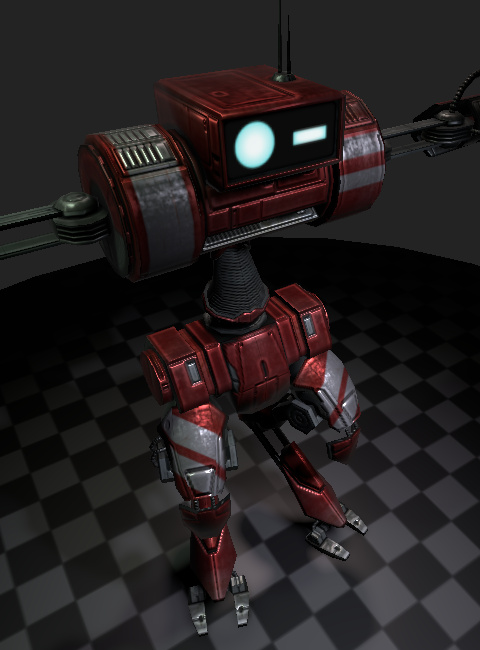
\includegraphics[width=0.45\linewidth]{./Figures/UBotPostOff.jpg}}
  \subfigure[Post-processing on]{\label{fig:UBotPostOn}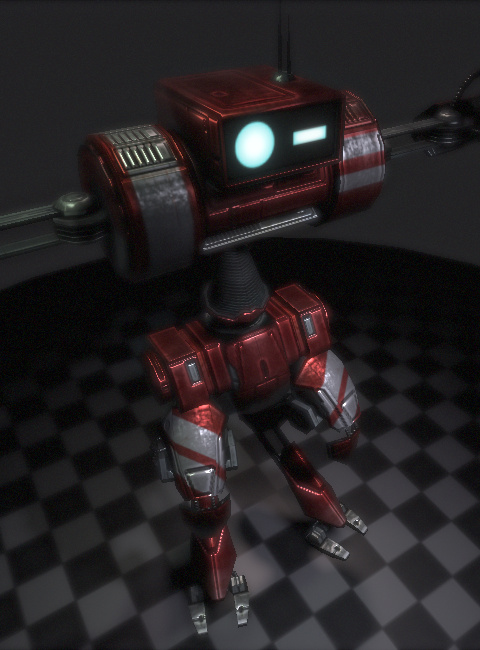
\includegraphics[width=0.45\linewidth]{./Figures/UBotPostOn.jpg}}
  \caption[The impact of post-processing]{The impact of post-processing on a rendered scene.}
\label{fig:lppFalloffBetterCase}
\end{figure}

\fref{fig:SimplePostProc} shows an example of a post-processing pipeline. The crucial item to notice in this graph is the \textbf{Blit} node. It is not a concrete kernel with an implementation in code, but a special entity which only the \emph{PostProcessor} understands. Such nodes are used to break the graph to be rendered in multiple passes. Since certain classes of image convolution operators are \emph{linearly separable}, they may be applied to a two-dimensional image as two single-dimensional operations. This is just what happens in this graph. Had the \emph{Blit} node been removed, the pipeline would implement a regular two-dimensional blur. With the \emph{Blit} in place, an equivalent operation \emph{(for all practical purposes)} is done an order of magnitude more efficiently. \fref{fig:SimplePostProcBreakdown} demonstrates the rendering steps which the graph from \fref{fig:SimplePostProc} is broken down into.

\begin{figure}[ht!]
  \centering
  \subfigure[The source pipeline]{\label{fig:SimplePostProc}\digraph[width=0.9\linewidth]{SimplePostProc}{
		"Blit" [
			fillcolor = "\#d0ffd0"
		];
		"Input" -> "Horizontal Blur";
		"Horizontal Blur" -> "Blit";
		"Blit" -> "Vertical Blur";
		"Vertical Blur" -> "Combine";
		"Input" -> "Combine";
	}}
  \subfigure[Breakdown into rendering passes]{\label{fig:SimplePostProcBreakdown}\digraph[width=0.6\linewidth]{SimplePostProcBreakdown}{
		subgraph "cluster_Pass1" {
			label = "Pass 1"
			"Blur1";
		}
		subgraph "cluster_Pass2" {
			label = "Pass 2"
			"Blur2";
			"Combine";
		}
		"Input" -> "Blur1";
		"Blur1" -> "Blur2";
		"Blur2" -> "Combine";
		"Input" -> "Combine";
	}}
  \caption[Simple post-processing with breakdown]{A simple post-processing pipeline.}
\label{fig:SimplePostProcWithBreakdown}
\end{figure}

In addition to causing multi-pass rendering, \emph{Blit} nodes may be used to rescale the images and change their internal format. A simple extension of the post-processing kernel shown in \fref{fig:SimplePostProc} could decide to output an image shrunk by 50\% on each side. With a sufficiently wide blur kernel, high-frequency details are lost anyway, so the signal may be represented by a smaller image within reasonable accuracy. Furthermore, combining the operator with itself a few times will approximate a blur with a very wide kernel in a much faster manner than a constant-resolution filter might.

\begin{figure}[ht!]
  \centering
    \digraph[width=0.7\linewidth]{PostProcMRT}{
		"Input";
		subgraph "cluster_MRT" {
			label = "rendered simultaneously"
			"Calc1";
			"Calc2";
			"Blit1" [ label = "Blit" fillcolor = "\#d0ffd0" ];
			"Blit2" [ label = "Blit" fillcolor = "\#d0ffd0" ];
		}
		"Calc3";
		"Input" -> "Calc1";
		"Input" -> "Calc2";
		"Calc1" -> "Blit1";
		"Calc2" -> "Blit2";
		"Blit1" -> "Calc3";
		"Blit2" -> "Calc3";
		"Calc3" -> "Output";
	}
    \caption[MRT usage in post-processing]{A simple post-processing pipeline in which multiple operations may be processed in the same pass through the usage of the \emph{Multiple Render Targets} functionality of GPUs.}
  \label{fig:PostProcMRT}
\end{figure}

When breaking down the post-processing pipeline into multiple passes, Nucleus will attempt to merge compatible and legal operations into a single pass via \emph{Multiple Render Targets} (\textbf{MRT}). An example is given in \fref{fig:PostProcMRT}. In this case, multiple textures are attached to a single framebuffer and their values are written by outputting a matching count of colors from the generated fragment shader. The legality is determined by the topological ordering of filters, as well as by considering the limitations of \emph{MRT}. For example, current GPUs require that all render targets have the same dimensions.

% TODO: describe the algorithm for breaking down processing into passes

\section{Functional composition}
\label{sec:FunctionalComposition}

The post-processing framework required an introduction of one more element into the type system and graph manipulation toolbox. A limitation of the kernel pipeline described so far is that each kernel produces a single set of outputs for a single set of outputs. While this restriction is reasonable for implementing structure, material, light and reflectance shaders, it hinders elegant image processing.

Consider the post-processing pipeline presented in \fref{fig:TrickyPostProc}. The \textbf{Blur} kernel expects to receive an image which it may sample multiple times, with various offsets. Connecting the \emph{Input} directly to \emph{Blur} would have worked fine within the framework described so far. However, in this particular case, the user decided to filter the input image through a power function first. The function is not specialized to work on images, but on individual values. There is a clear type mismatch, but intuitively this case should work just fine.

\begin{figure}[ht!]
  \centering
    \digraph[width=0.7\linewidth]{TrickyPostProc}{
		"Image" -> "pow2 (in float4, out float4)";
		"pow2 (in float4, out float4)" -> "Blur (in Image)";
	}
    \caption[A tricky post-processing pipeline]{A tricky post-processing pipeline}
  \label{fig:TrickyPostProc}
\end{figure}

The key to solving this issue lies in realizing what exactly is an image. In the particular case of shading languages, the answer is simple: it is a function of two-dimensional coordinates into colors, or more specifically, $float2 \Rightarrow float4$. If $input$ is the original image and $pow2$ is the power function, then what we really need to do is provide the $pow2 \circ input$ function to the \emph{Blur} kernel. This \emph{functional composition} is automatically performed by Nucleus.

Kernels within Nucleus are technically functions, so unsurprisingly, the \emph{Image} type seen in the aforementioned example is indeed a kernel; particularly, one with the following signature:
	
\noindent\begin{minipage}{\textwidth}
\begin{lstlisting}[frame=single]
Image = kernel(
    in uv <type float2 + use uv>,
    out sample <type float4 + use color>
);
\end{lstlisting}
\end{minipage}

The \emph{Blur} kernel in \fref{fig:TrickyPostProc} expects a \emph{kernel} as its input (it also expects two more parameters, which are irrelevant to the example), but the parameter connected to this input is not a kernel. Its type, however, is the type of the kernel's \emph{output} (\emph{float4}). Moreover, the incoming subgraph contains a free ``float2 uv'' parameter, which is exactly what the \emph{Image} kernel needs. Hence despite the type mismatch, the entire subgraph connected to the final \emph{Blur} node can be converted to an \emph{Image}.

\begin{figure}[ht!]
  \centering
    \digraph[width=0.8\linewidth]{TrickyPostProcResolve}{
		subgraph "cluster" {
			label = "function (in uv <type float2>, out sample <type float4>)"
			"uv" [ fillcolor = "\#909090" ];
			"Image";
			"pow2";
			"sample"  [ fillcolor = "\#909090" ];
		}
		"uv" -> "Image";
		"Image" -> "pow2";
		"pow2" -> "sample";
		"sample" -> "Blur";
	}
    \caption[The tricky post-processing pipeline resolved]{The tricky post-processing pipeline from \fref{fig:TrickyPostProc} resolved via functional composition}
  \label{fig:TrickyPostProcResolve}
\end{figure}

More specifically, when the kernel graph contains a connection from an output of type $V$ to an input of type $F = (P \rightarrow O)$, $V \neq F$, such that $c_O : V \rightarrow O$ is a valid conversion within the semantic type system, the coercion algorithm will attempt to perform functional composition of kernels. In order for it to succeed, the incoming subgraph from which the $V$-typed output came must contain a free parameter of type $I$ such that $c_I : P \rightarrow I$ is a valid conversion within the semantic type system.

Any kernel subgraph may be considered a function. Let $g$ be the incoming subgraph from the aforementioned example. If the criteria for kernel composition are satisfied, it is possible to construct a function $g\prime : P \rightarrow O = c_O \circ g \circ c_I$. This function is hence provided to the (higher-order) destination kernel and type coercion is complete.

Substituting $float2$ for $P$ and $I$, $float4$ for $O$ and $V$, as well as the identity function for $c_O$ and $c_I$, the particular example with image blurring from \fref{fig:TrickyPostProc} is achieved. The result is shown in \fref{fig:TrickyPostProcResolve}.

A requirement for functional composition is that the incoming subgraph contains free parameters. In order to prevent automatic flow determination from connecting anything to parameters meant to be used in composition, graph inputs may be marked to opt-out of automatic data flow. The kernel definition \emph{domain-specific language} provides a handy annotation to be used for this purpose.

%TODO
%More specifically, given a higher-order function $f : (A \rightarrow B) \rightarrow C$, and functions $g : D \rightarrow B$ and $h : A \rightarrow D$, the type system recognizes the invalid application $f(g(h))$, and turns it into $f(g \circ h)$.

Overall, the functional composition algorithm allows for a natural extension of graph-based processing, reducing the restriction of linear data flow in the \emph{DAG}, while still retaining functional purity, important for easy reasoning about and optimizations of the generated code. Conceptually, this feature is similar to automatic ``lifting'' of functions in some programming languages natively supporting arrays, such as \emph{APL} and \emph{J}.

Naturally this very mechanism is not restricted to just the post-processing component of Nucleus and may be used e.g. in order to implement procedural texturing. In this case, the \emph{Image} kernel will abstract away regular texture access and procedural texture generation, providing an unified interface over them without any runtime overhead.
% TODO: ref the blurred checker example
	
\section{Code generation}
\label{sec:codegen}

Before anything can be rendered via kernels, they need to be translated to a form which a low-level rendering API (and hence the GPU) understands. This is done by generating shader code. The input to this final pass (henceforth called \emph{codegen}) is a complete kernel graph, with all conversions resolved and automatic flow deduced. Given this graph, the first step is determining which of its parts should run in which stages of the rasterization process.

A vertex shader processes each vertex in isolation and has a single mandatory output - the clip space position of the vertex. Such transformed vertex is then used by the primitive assembly stage of the GPU, which subsequently proceeds to scan-line conversion. Attributes output by the vertex shader are linearly interpolated across the primitive and made available to the fragment shader. The key observation here is that only the vertex position is special and must be made available in a particular format. All other outputs of the vertex shader are simply parameters which the fragment shader needs to generate the final color. It is then safe to assume that all computations of the kernel graph except the position may be done in the fragment stage. This assumption translates directly into the first step of the algorithm which determines the domain of each concrete kernel node:

\begin{enumerate}
\item Assume all nodes should run in the fragment domain.
\item Find a specially designated \textbf{Rasterize} node, mark it and all of the nodes in its incoming subgraph to run in the vertex domain.
\end{enumerate}

The \textbf{Rasterize} node is normally a part of a \emph{Structure} kernel graph specified for a renderable, but any node which accepts a position parameter may be used instead if a custom \emph{Renderer} deems it necessary. Due to the semantic type system, any data convertible to a clip space position may be supplied as the input.

Functions defined within the semantic type system do not need their storage types to be defined -- for example, an addition kernel should work on vectors, scalars and matrices, therefore it is a generic function. The type for its parameters is determined within the coercion mechanism described in \sref{sec:TypeCoercion}. Therefore it may happen that the same kernel has to be generated in multiple instances, with types specialized for each fully coerced type. The code generation step resolves this gracefully by renaming functions in the target language and substituting types within the declarations.

Since graph-based kernels building up the final kernel graph for which codegen runs, the graph being compiled consists of only code-based kernels. Therefore it emits the code-based kernels as functions in the target language (\emph{Cg} currently) and creates glue code within entry points for each shader domain. The generated glue may look like:

\noindent\begin{minipage}{\textwidth}
\begin{lstlisting}[frame=single]
void FragmentProgram (
	in float2 n4__uv : TEXCOORD,
	out float4 bridge__0 : COLOR
) {
	Image n11__image;
	SamplerToImage(
		in__0tex,
		n11__image
	);
	// ...
	float4 n12__output;
	Blit_frag(
		n6__kernel,
		n4__uv,
		n12__output
	);
	bridge__0 = n12__output;
}
\end{lstlisting}
\end{minipage}

That is, \textbf{out} parameters are declared before each kernel function call, then passed to subsequent calls as arguments. At the end of the generated function, its outputs are gathered from the temporary variables created within the generated glue code, as can be seen in the last line of ``FragmentProgram'' in the above example. The extra variables and function calls only exist in the semantic phase of the high-level shading language compiler (\emph{cgc} in this case), but are inlined in the generated code, therefore do not cause any slowdown or bloat at runtime.

\subsection{Optimization due to linear functions}

The presented assignment of computational nodes to GPU domains is sufficient but not optimal. A typical scene rendering processes more fragments than vertices, so it is desirable to move calculations from the fragment to the vertex stage where possible. In order to show how this is possible, it is convenient to take a closer look at the vertex and pixel processing pipeline from a mathematical point of view. Due to machine precision limits, the following consideration is strictly correct, but suffices for all practical purposes.

Let $f$ be the fragment shader, $v$ the vertex shader and $p_0 p_1 p_2$ the triangle being rasterized. The GPU computes $f(w_0 v(p_0) + w_1 v(p_1) + w_2 v(p_2))$ for each pixel of the triangle, where $w_0$, $w_1$ and $w_2$ are the barycentric coordinates of the center of the pixel with respect to $p_0 p_1 p_2$. Let now $g$ and $h$ be functions so that $h$ is linear and $g \circ h = f$. \\
Because $h$ is linear, \\
$g(h(w_0 v(p_0) + w_1 v(p_1) + w_2 v(p_2))) = g(w_0 h(v(p_0)) + w_1 h(v(p_1)) + w_2 h(v(p_2))$.

Subsequently, we can define a vertex shader function $v\prime = h \circ v$ and a fragment shader function $f\prime = g$. This result shows that it is legal to move a kernel from the fragment stage to the vertex stage as long as all of its inputs come from the vertex stage and the kernel implements a linear function. By utilizing this rule repeatedly in topological order, the process can be done in a single pass for the entire kernel graph. Nucleus currently allows a kernel to be tagged as linear, however in a future implementation this may be inferred automatically through semantic analysis of the code.

\begin{figure}[ht!]
  \centering
  \subfigure{\label{fig:linFuncOpt1}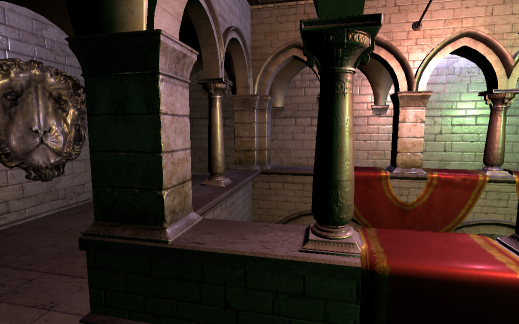
\includegraphics[width=0.4\linewidth]{./Chapters/linearOptScr1.jpg}}
  \subfigure{\label{fig:linFuncOpt2}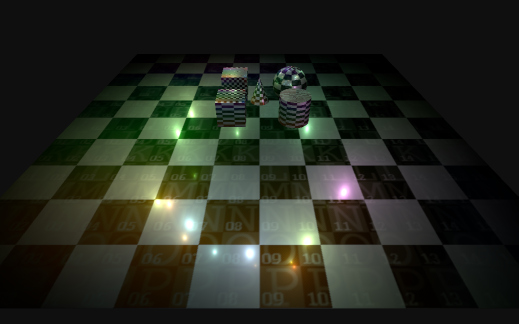
\includegraphics[width=0.4\linewidth]{./Chapters/linearOptScr2.jpg}}
  \caption{Scenes used to test the speedup from optimization due to linear functions}
  \label{fig:linFuncOpt}
\end{figure}

\fref{fig:linFuncOpt} shows two scenes, which render respectively at 93 and 131 FPS without the optimization step. With it enabled, the performance reaches 96 FPS and 133 FPS respectively.

\subsection{Code generation for functional composition}

Functional composition does not require anything special from kernels, aside from them having the proper signatures. For instance, given the following ``Image'' kernel:

\noindent\begin{minipage}{\textwidth}
\begin{lstlisting}[frame=single]
Image = kernel(
    in uv <type float2 + use uv>,
    out sample <type float4 + use color>
);
\end{lstlisting}
\end{minipage}

One could construct a kernel which uses it like so:

\noindent\begin{minipage}{\textwidth}
\begin{lstlisting}[frame=single]
SampleImage = kernel (
	in image <type Image>,
	in uv <type float2 + use uv>,
	out sample <use color + in.image.actual + type float4>
) {
	sample = image.sample(uv);
};
\end{lstlisting}
\end{minipage}

Inline code within non-graph kernel bodies must be valid for the target language as to be emitted literally during the codegen process. Therefore the ``image.sample(uv)'' expression must be valid inside the generated function. This is an aspect which is not entirely satisfactory, because it ties some constructs of kernel implementations to the target language used during code generation. In this particular case, it requires that the target language supports method calls or expressions which look like them. If generalization to other shading languages is required, a more sophisticated codegen process may be used, however for the purposes of this thesis, \emph{Cg} is assumed.

In order for expressions using kernels to be valid in \emph{Cg}, \emph{interfaces} are generated. In the above case, the following interface would be defined:

\noindent\begin{minipage}{\textwidth}
\begin{lstlisting}[frame=single]
interface Image {
	float4 sample(float2 uv);
};
\end{lstlisting}
\end{minipage}

With this in place, the actual work done within functional composition may be hidden behind a concrete implementation of such an interface. For example, an implementation which returns blurred samples of another \emph{Image} might be emitted as:

\noindent\begin{minipage}{\textwidth}
\begin{lstlisting}[frame=single]
struct Image__impl6_g0 : Image {
	// ...
	float4 sample(float2 uv) {
		float4 n3__sample;
		BlurImage4__overload0_g1(
			uv,
			// ...
			n3__sample
		);
		return n3__sample;
	}
};
\end{lstlisting}
\end{minipage}

Again, interfaces only exist during semantic analysis of the code in \emph{Cg} and do not cause any overhead at runtime, which would be present in languages such as Java. Therefore the functional composition mechanism is a robust extension of linear data flow in a graph-based shading system.
 % Nucleus
% Chapter 5

\chapter{ Nucled }
\label{Chapter5}
\lhead{Chapter 5. \emph{ Nucled }}

The entire machinery of Nucleus may be operated from source code and configuration files. While the \emph{ domain specific language } created for this purpose makes it possible and relatively easy, real-world usage scenarios demand a more intuitive solution. The obvious one for Nucleus was to use a graph-based visual design tool, similar to the ones used by [TODO: refs].

I have created such a tool, dubbed "Nucled". While it's not yet feature-complete, its capabilities include:

\begin{itemize}
\item kernel graph creation and manipulation
\item editing of the Cg source code of kernels,
\item real-time preview of graphical effects,
\item manipulation of 3D scenes,
\item application and creation of new materials,
\item manipulation of post-processing pipelines.
\end{itemize}

The interface of Nucled is based on a custom Graphical User Interface (GUI) toolkit \cite{HybridGUI}, which is able to use the low-level layer of Nucleus as the display backend. This approach guarantees smooth integration of the rendering framework within Nucled and serves as a test of the system. While the editor looks like a regular desktop application, it's in fact rendered entirely by Nucleus, down from each button, text label, up to 3D scene viewports and material previews.

The machinery of material previews.

Some info about how post-processing previews are displayed.

Info about the issues mentioned by Whitted (mentioned in McGuire's paper) about type mismatches and how they're mostly non-existent in Nucled thanks to the semantic type system.

Mini-conclusion as how Nucled is a sketch but may become a complete solution for authoring effects.
 % Nucled
% Chapter 6

\chapter{ Examples }
\label{Chapter6}
\lhead{Chapter 6. \emph{ Examples }}


\section{Implemented reflectance models}
\section{Forward rendering}
\section{Deferred rendering}
\section{Shadows}
\section{Post-processing effects} % Examples
% Chapter 7

\chapter{ Conclusions }
\label{Chapter7}
\lhead{Chapter 7. \emph{ Conclusions }}

The main contribution of this thesis is a rendering system whose building blocks at several scales are freely reusable in the context of rendering effects and algorithms. The presented framework is built on top of standard rendering facilities supported by graphics hardware, and therefore does not sacrifice performance. At the same time, it provides an intuitive level to program for, similar in many aspects to the field-tested design of \emph{RenderMan}. The high level building blocks of \emph{kernels} can be used throughout the system and have been demonstrated to work in \emph{forward}, \emph{deferred} and \emph{post-processing} pipelines. On the other hand, the low level elements completely abstract away the underlying graphics API and supplement the system with trivial rendering operations, whenever the kernel-based counterpart is not satisfactory or desired.

Due to the implementation of a semantically-rich type system over computational elements, the burden of mundane representation and basis conversion of data has been considerably lifted, therefore improving workflow and reducing the possibility of introducing errors.

The system presented in this thesis has been verified by implementing numerous rendering techniques on top of and through its primitives. Additionally, a graphical authoring tool has been presented, building on the framework and being able to feed data back into itself via an easy to use interface.

\section{Future work}

Despite all the work poured into it, Nucleus is still only the beginning of a rendering system which might be used in a game or for complex visualization purposes. Therefore the potential ways to expand it are vast, ranging from simple refactoring to optimization via complex algorithms such as Tiled Deferred Rendering \cite{tiledDeferred}. Most critically, it lacks several important features omitted entirely in this thesis, e.g.:
\begin{itemize}
\item Hidden surface removal (the implementation contains stubs for it and uses only view frustum culling),
\item Character animation,
\item Particle system simulation and rendering,
\item Run-time background streaming of assets.
\end{itemize}

The aforementioned functionality would be implemented either on top of the existing framework or beside it. At the same time, existing features may be improved upon as well. First and foremost, the kernel authoring tool, \emph{Nucled}, is in dire need of improvements. The groundwork has been laid, but before it becomes a full-fledged editor, it needs better error handling, more detailed previews, support for arbitrary manipulation of loaded scenes and proper management of asset libraries.

Beside \emph{Nucled}, the very core of the system requires further work. \emph{Semantic expressions} have been added during late development stages of Nucleus, and while very useful, they only point out that a more flexible, generic type system would be beneficial. In particular, it is not currently possible to define a function, constraining some of its parameters to the same value of a trait, without specifying what this value is. For example, stating that the parameters should all come from the same coordinate system, but allowing it to be generic instead of specifying e.g. ``local'' or ``world''. Currently, the only way to do this is via code duplication. Perhaps even more importantly, the type system should be rigorously defined in terms of programming language theory, as the current implementation is very much ad-hoc.

Lastly, a potential area of future research lies in determining how the presented system might be extended to support hardware tessellation introduced in \emph{Shader Model 5} \cite{SM5}.
 % Conclusion
% Chapter 8

\chapter{ Future work }
\label{Chapter8}
\lhead{Chapter 8. \emph{ Future work }}

TODO: 

\section{Tiled deferred}
\section{Custom shading language with semantic types}
\section{Shader LoD}
 % Future work

%% ----------------------------------------------------------------
% Now begin the Appendices, including them as separate files

\addtocontents{toc}{\vspace{2em}} % Add a gap in the Contents, for aesthetics

\appendix % Cue to tell LaTeX that the following 'chapters' are Appendices

%\input{./Appendices/AppendixA}	% Appendix Title

%\input{./Appendices/AppendixB} % Appendix Title

%\input{./Appendices/AppendixC} % Appendix Title

\addtocontents{toc}{\vspace{2em}}  % Add a gap in the Contents, for aesthetics
\backmatter

%% ----------------------------------------------------------------
% \label{Bibliography}
% \lhead{\emph{Bibliography}}  % Change the left side page header to "Bibliography"
% \bibliographystyle{unsrtnat}  % Use the "unsrtnat" BibTeX style for formatting the Bibliography
% \bibliography{Bibliography}  % The references (bibliography) information are stored in the file named "Bibliography.bib"

\end{document}  % The End
%% ----------------------------------------------------------------
